\documentclass{article}
\usepackage[utf8]{inputenc}
\usepackage[T1]{fontenc}
\usepackage{subfig}
\usepackage{amsmath,amssymb}
\usepackage{mathabx}
\usepackage{adjustbox}
\title{Engineer's Thesis}
\author{Wojciech Pratkowiecki}
\date{December 2018}

\usepackage{natbib}
\usepackage{graphicx}

\begin{document}

\maketitle

\section{[PL] Konspekt}
Poznanie faktycznego rozkładu obu chmur punktów mogłoby pomóc w zrozumieniu działania zarówno GRL jak i powodu niepowodzeń przy użyciu konceptorów. Dodatkowo sama natura problemu adaptacji dziedzinowej mogłaby stać się znacznie bardziej zrozumiała. Z tego powodu postanowiliśmy w znacznym stopni ograniczyć wymiarowość D wyjścia feature extracotra, ustawiając $D=3$. Dzięki temu zabiegowi wejście do naszego modelu jest mapowane na 3 liczby, możemy zatem je zobrazować w 3 wymiarowym układzie współrzęnych. W ten sposób otrzymamy faktyczny wygląd chmury punktów wyznaczonej przez obie dziedziny po przekształceniu przez feature extracotr. Sekcja Visualization zawiera szczegółowy opis eksperymentu wraz z wynikami.
\par
Tak drastyczne zmniejszenie wymiarowości wyjścia feature extracotra odbija się negatywnie na wyniku adaptacji dziedzinowej, model z GRL uzyskuje gorze wyniki od tradycyjnej sieci klasyfikującej MNIST bez dostosowywania jej do innej dziedziny. Jednocześnie wizualizacje jakie umożliwia wartstwa rozmiaru 3 wydają się bardzo przydatnym narzędziem w analizie działania GRL. Aby nie rezygnować z możliwości wizualizacji danych, ale jednocześnie umożliwić feature extractorowi generowanie bardziej skomplikowanej reprezentacji danych, co również da większe pole do popisu GRL, możemy zmienić architekturę modelu, przywracając oryginalny feature extractor mapujący punkty wejściowe do wielowymiarowej przestrzeni $\mathbb{R}^{D}$, a modyfikując predyktor klasy, dodając na jego początek warstwę transformujacą dane do 3 wymiarów. Dzięki temu nadal możemy wizualizować nasze dane poprzez przekształcenie obrazka wejściowego przez feature extractor oraz pierwszą warstwę klasyfikatora, jednocześnie umożliwiając GRL działanie z bardziej skomplikowaną reprezentacją danych. Model o tej budowie osiąga znacznie lepszy wynik w klasyfikowaniu danych z dziedziny docelowej - ma ok. 70\% skuteczności. Jednocześnie wizualizacje, jakie otrzymujemy przez naniesienie na układ współrzędnych nowej reprezentacji danych są bardzo podobne do tych, które otrzymaliśmy w poprzednim rozdziale.
\par
Otrzymane wizualizacje potwierdzają rozłożenie punktów w postać wieloramiennej gwiazdy. Aby potwierdzić nasze intuicje odnośnie przyczyn problemów w klasyfikacji części przykładów możemy sprawdzić, gdzie leżą punkty, które klasyfikujemy poprawnie z najwyższą pewnością, a gdzie te, co do których się mylimy. Wizualizacja pokazuje, że przykłady które sklasyfikowaliśmy źle są przez feature extractor wraz z pierwszą warstwą predyktora klasy mapowane w pobliże środka układu współrzędnych, gdzie wymieszane są ze sobą mapowania punktów z różnych klas, rzadko kiedy mylimy się co do punktów leżących odlegle od środka układu. Model jest natomiast najpewniejszy dla punktów położonych w ramionach otrzymanej gwiazdy, co wydaje się logicznym wynikiem. Dodatkowo możemy podjąć próbę zwizualizowania konceptora dla reprezentacji otrzymanej przez feature exrtactor. Jako, że jest on elipsoidą w wielowymiarowej przestrzni nie możemy tego zrobić wprost, jednkaże dobrym wyjściem wydaje się losowanie punktów w $\mathbb{R}^{D}$ i sprawdzanie, czy leżą one wewnątrz elipsoidy. Następnie pierwszą warstwą predyktora klasy mapujemy do $\mathbb{R}^{3}$ te punkty, które znajdowały się wewnątrz wyznaczonej przez konceptor elipsoidy. Dzięki zastosowaniu mniejszej sieci, a także wprowadzeniu regularyzacji, quota konceptora nie wynosi już 99\%, nasza elipsoida zajmuje teraz 85\% przestrzeni. Wizualizacja pokazuje, że punkty, które leżą wewnątrz konceptora układają się w elipsoidę i faktycznie nie wyglądają jak kula zajmująca całą przestrzeń. Jednakże próby zastosowania konceptorów w celu adaptacji dziedzinowej nie powiodły się, a same konceptory stały się dla nas niewiele bardziej zrozumiałe.
\par
Aby zwizualizować nasze dane nie jest konieczne używanie warstwy rozmiaru 3 w architekturze modelu. Z pomocą przychodzą nam różne metody redukcji wymiarowości, takie jak PCA. Metody te polegają głównie na rzutowaniu danych na pewne wektory własne macierzy wyznaczonej przez punkty danych. Aby uzyskać możliwie najlepszą redukcję wymiarowości wybieramy wektory własne odpowiadające największym wartościom własnym. Aby móc zwizualizować dane musimy ograniczyć nasze D wymiarów do zaledwie trzech. Jeżeli spojrzymy na wartości własne macierzy uzyskanej przez transformację zbioru wejściowego przez feature extractor zobaczymy, że trzy największe z nich nie odbiegają wielkością od kilku pozostałych. Oznacza to, że redukcja do3 wymiarów mocno zniekształca obraz danych. Jest to również potwierdzenie, że problem ten nie jest mozliwy do prostego rozwiązania z użyciem 3-wymiarowego wyjścia feature extracotra. Wizualizaje przy użyciu metod takich jak PCA czy KernelPCA nie są tak interesujące jak te z użyciem warstwy rozmiaru 3 wewnątrz sieci neuronowej, jadnak nadal pokazują, że użycie GRL pomaga w nałożeniu się na siebie chmur punktów dla obu dziedzin.

\begin{abstract}
The amount of data that is still unlabeled has been growing over recent years. With domain adaptation methods it is possible to get a model that classifies well these samples, if only a related and labeled set is available. Therefore, the popularity of domain adaptation has strongly increased. While trying to get better and better results, many diverse and complex approaches were invented. This paper describes researches and experiments aimed at understanding the problem of domain adaptation and coping with it using the Gradient Reversal Layer.
\end{abstract}

\section{Introduction}
Neural networks have found many applications in recent years due to their ability of learning some complex data dependencies. Top performance in various tasks have resulted in increased popularity of not only neural networks and deep learning but also of other machine learning (ML) methods. Different architectures designed for different tasks were invented. One of them is convolutional neural network (CNN), which caused huge improvement in the image classification field. However, obtaining top-performing models often requires a long training, with huge amount of labeled data. Such a complicated procedure yields a desired model, but it would not reach comparable results on different, even strongly related dataset. Moreover, if we  have small amount of labeled samples, we need to find an alternative way to train the network. At this point domain adaptation is an attractive option.
\par
Domain adaptation (DA) is a process of learning a distribution of samples from source domain and obtain a model that performs well on other, but related, target domain. For instance, if we have a huge (e.g. synthetic), labeled set of road signs images and a video from a ride through a city, we could get an effective model that classifies well all the signs from the video frames, if we train it properly with the labeled dataset. One of domain adaptation techniques is the Gradient Reversal Layer (GRL) proposed by Yaroslav Ganin and Victor Lempitsky. GRL is a simple, but effective, architectural trick, applied during backpropagation, designed especially for domain adaptation task. This thesis is a collection of researches on the Gradient Reversal Layer and its adjustments. I tried not only to improve the results but also to get a detailed understanding of domain adaptation problem and GRL behaviour.

\section{Theoretical framework}
\subsection{Artificial neural network}

Artificial neural network (ANN) is a machine learning technique inspired by neural connections in human brain. While training the model we use a pre-defined architecture and loss function. The architecture describes the transformation of the input data made by our model, its complexity and interpretation of the output. Each network contains neurons that are stacked in layers. Neurons are nothing but a weighted sum characterized by neuron's weights and bias. A layer is built with many neurons and followed by non-linear activation function. Each layer transforms its input vector into an output vector. The first layer of the network is called the input layer, the last one is the output layer, while all the intermediate layers are called hidden layers. Figure~\ref{fig:ANN} presents a sample ANN. The loss function is a way to measure and optimize the performance of the model, it is commonly the magnitude of its imprecision. 
\par
Successful learning process requires many examples of the problem we want the network to solve. At the beginning, we usually set the model's parameters (mostly denoted as $\Theta$) to random values. The model transforms some of the input examples and we compute the loss function based on the output. As we want the model to perform as well as possible, our goal is to minimize the loss function. Therefore we use the backpropagation method - for each input sample we compute its gradient. The values of those gradients tell us, how should we tune model's parameters $\Theta$ to find the minimum of loss function. Therefore, we slightly change values of $\Theta$ in the direction of gradient, which should recall in a better performance of the model on the next examples. We repeat this process many times, improving our network during whole learning process. 
\par
This iterative training approach is a simplified description of stochastic gradient descent (SGD) - one of the most popular and effective ANN optimization method. As our model may be defined by millions of parameters, computational cost of thousands of training iterations is a huge drawback of neural networks. However, great growth of computer's computation power with GPU acceleration let us find solutions for some really complex problems within decent time.  Therefore neural networks are nowadays widely used for many tasks. One of them is image classification - finding for a given input image the most likely label from a fixed label set.

\subsection{Convolutional neural networks}
Applying neural networks to image processing became very popular. To keep reaching better results in tasks like image classification some new inventions were needed. The breakthrough came with convolutional neural networks (CNN). CNN, just like classical neural network, is built with neurons stacked in layers. First layers of CNN are convolution layers. Each of them is a set of learnable, small size (like 5$\times$5) filters followed by activation function. Each filter processes input image step by step and produces a transformed, usually smaller, one. Therefore after each layer we get a new set of images obtained from all pictures from previous layer. A big advantage of this approach is a much smaller number of learnable parameters - if the input image has size 1000 $\times$ 1000 it would require 1000000 parameters for a single neuron in a fully connected layer, while convolution layer processes it with its filter, that has 25 parameters, if the size of the filter is 5$\times$5.  After a convolution layer we usually use pooling - we divide the picture into cells (e.g. of size 2$\times$2) and we replace the whole cell with its maximum value (in case of maximum pooling). This operation reduces the size of the image internal representation, and force the network to focus on important patterns. Figure~\ref{fig:CNN} presents an example of CNN architecture.
\par
The convolutional part of the model learns high-level features or descriptors of locations in the input image. Moreover it makes the network invariant for small translation of object over the image. If our model classifies dog breeds, it will give the same result, no matter if the dog is in the middle or in a corner of the photo. Convolutional layers produce a vector representation of the input image. It is then fed into classical, fully-connected layers that return the model's output. If our task is image classification the output is a vector of classes probabilities typically.
\par
CNNs caused huge improvements in both accuracy and speed of image classification. Nowadays top-performing architectures in many image processing problems are built with convolutions. Convolutional layers also found application in some non-picture field like some natural language processing tasks or speech generation. 

\begin{figure}[htb]%
    \centering
    \includegraphics[width=\linewidth]{ANN.jpeg}%
    \caption{Example of neural network architecture}%
    \label{fig:ANN}%
\end{figure}
\begin{figure}[htb]%
    \centering
    \includegraphics[width=\linewidth]{CNN.png}%
    \caption{Example of convolutional neural network architecture}%
    \label{fig:CNN}%
\end{figure}

\subsection{Digit classification with CNN}
One of the most famous dataset in machine learning is MNIST - a collection of black and white photos of handwritten digits. Every picture's resolution is 28$\times$28 pixels, each one is an integer in the range $[0,255]$, that describes the brightness of the pixel. All the samples are provided with ground truth labels. Classification of digit images is therefore a task of processing the input image that dimensionality is 28$\times$28, and assigning probabilities for each of 0-9 digits. The model prediction is the digit with highest probability. Even very ordinary convolutional architecture reaches over 99\% accuracy on this dataset. A bit more challenging modification of MNIST is the MNIST-M set, obtained by blending example from MNIST with some color photos from BSDS500. There is probably no difference in difficulty of classification MNIST and MNIST-M digits for human, but from neural network point of view, the colorful set is much more complex. Nevertheless, obtaining top-performing model is relatively easy.
\par
There are a lot of similar digit recognition datasets, with many that are much more complex than MNIST and its modifications. The Street View House Number (SVHN) is a good example of such collection. SVHN samples are obtained from Google Street View photos, therefore they are colorful, with diverse backgrounds, pictures are often blurry and a single image may present few digits, while its label is the one in the centre of the photo. Due to all those properties of SVHN, model that classifies well its samples must be complex and longer trained. 
\par
Even though digit classification seems not to be the most important and entertaining problem that CNN may solve, it is still one of the most popular field of measuring a model's performance and yields experimental results with quick turn-around time. Figure~\ref{fig:digits} presents some examples from mentioned datasets - MNIST, MNIST-M and SVHN.

\begin{figure}%
    \centering
    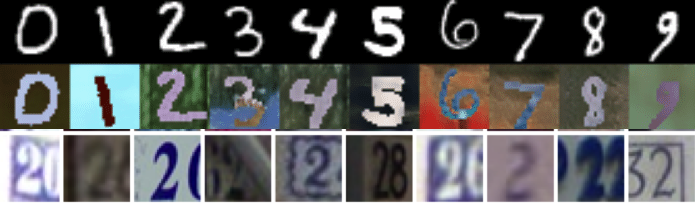
\includegraphics[width=\linewidth]{digits.png}%
    \caption{Samples from MNIST, MNIST-M and SVHN digit images datasets, best viewed in color}
    \label{fig:digits}%
\end{figure}

\subsection{Domain adaptation}
Let's suppose that we have a novel, large set of digit images, for instance photos of the back of each European footballer's jersey, preprocessed in a way, that every image contains one digit - figure~\ref{fig:football} presents some possible samples. Our goal is to obtain a model that classifies digits from football kits. Unfortunately we don't have any labels for these pictures, so we are unable to go a straightforward way and train a CNN adjusted to the image set, as we cannot determinate if the model's prediction is right. In this kind of situation domain adaptation is a solution.
\par
Domain adaptation is a specific training process, when we teach a model with examples from a source domain, but our goal is to make it perform well on different, but related, target domain. Over recent years many architectures have been proposed to reach as high target domain accuracy as possible. DA is needed when samples from target distribution are unlabeled (unsupervised domain adaptation) or we have just few labeled examples (semi-supervised domain adaptation). A model should find a mapping between domains, which would allow source domain classifier perform well on test (target domain) examples.
\par
In our case of football jerseys, when the set is unlabeled at all, we have an unsupervised DA problem. Target domain is the distribution of jersey's photos. Now we should try to obtain a model learned with labeled examples from other dataset, like SVHN, and apply some architectural solution that would let the model classify well digits from football kits. Dozens of such tricks have been proposed in recent years. One of them is Gradient Reversal Layer.

\begin{figure}%
    \centering
    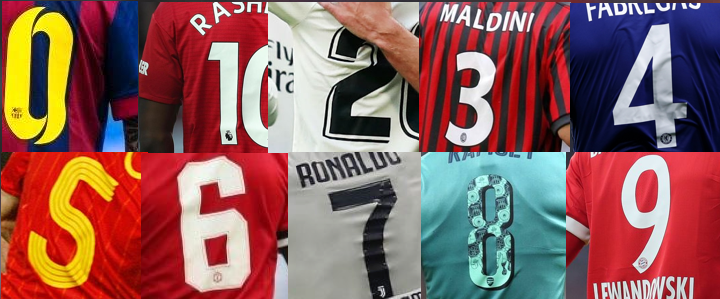
\includegraphics[width=\linewidth]{football.png}%
    \caption{Football jersey dataset}
    \label{fig:football}%
\end{figure}


\subsection{Gradient reversal layer}
Gradient Reversal Layer was introduced by Yaroslav Ganin and Victor Lempitsky in the paper titled "Unsupervised Domain Adaptation by Backpropagation" in 2015. The authors describe domain adaptation as a problem of finding common mapping for source and target distribution, that would transform samples to some kind of representation that allows classifier perform well and does not contain any information about the domain of mapped sample. In perfect scenario the mapping does not influence the label predictor's accuracy, but is so invariant w.r.t. domain shift that we cannot obtain a model, that predicts well the distribution of the input.
\par
Gradinet Reversal Layer itself is a simple trick used during backpropagation pass. It is a trival layer in network's architecture, that leaves the input unchanged during forward propagation, but multiplies the gradinet by negative scalar $\lambda$ during backpropagation. Formally we could say that GRL is a function specified as:
\begin{equation*}
GRL(x, \lambda) = \begin{cases}
x &\text{forward pass}\\
-\lambda \cdot x &\text{backward pass}
\end{cases}
\end{equation*}
GRL demands a special architecture, contructed with three parts - a \textit{feature extractor}, that is denoted as $G_{f}$ and maps the input to a $D$-dimensional vector $f \in \mathbb{R}^{D}$. Feature extractor is a neural network with its parameters $\Theta_{f}$, so the transformation of input vector $x$ is denoted as $G_{f}(x;\Theta_{f})$. This representation is then used by two other components of the model - a \textit{class predictor} $G_{y}$ with parameters $\Theta_{y}$, that classifies the $f = G_{f}(x;\Theta_{f})$ vector, 
and a \textit{domain predictor} $G_{d}$ with its parameters denoted as $\Theta_{d}$, which task is to predict the domain label of the vector $f$. The very first layer of $G_{d}$ is the GRL, therefore during backpropagation the gradient that comes to the feature extractor from domain predictor is multiplied by -$\lambda$. Figure~\ref{fig:GRLarch} presents a diagram with described architecture.
\par
All those three components are independent neural networks that construct our architecture. While training the model we aim to force $G_{f}$ to yield domain-invariant feature vectors $f$. GRL placed at the beginning of $G_{d}$ should be very helpful. The intuition behind inversion of the gradient sign during backpropagation is to follow the opposite direction to the domain predictor gradient, so after each update of the parameters of feature extractor, the feature vector $f$ should be more involved for $G_{d}$ and a good prediction of its domain label - much harder. $G_{d}$ itself tries to minimize its own loss function to make better predictions. If the domain predictor, that wants to does its best, is unable to determinate the distribution of the $f$, then $f$ is getting more domain-invariant. In perfect scenario GRL has such an impact on $\Theta_{f}$, that $G_{d}$ has the same accuracy as random model. Concurrently $G_{y}$ tries to predict a class of each sample and we try to minimize its loss function. Class predictor's gradient is used to tune $\Theta_{y}$ and then passed do feature extractor. Therefore the feature extractor's parameters are tuned w.r.t. gradient of $G_{y}$ and a negatively multiplied gradient of $G_{d}$. If we denote loss for class prediction as $L_{y}$ and loss for domain classification as $L_{d}$ then our goal is to minimize the function:
\begin{align*} 
E(\Theta_{f}, \Theta_{y}, \Theta_{d}) = &\sum_{\substack{i=1.N \\ d_{i}=0}} L_{y}(G_{y} (G_{f}(x_{i};\Theta_{f}); \Theta_{y} ), y_{i} ) - \\
 &\lambda \cdot \sum_{\substack{i=1.N \\ d_{i}=0,1}} L_{d}(G_{d} (G_{f}(x_{i};\Theta_{f}); \Theta_{d} ), d_{i} )
\end{align*}
where $(x_{i}, y_{i})$ are samples from $d_{i}$ and values $i$ of $d_{i}$ are 0 for source domain and 1 for target domain. Label predictor $G_{y}$ does not classify samples from target domain (as we don't have labels for them), so during the training this part of architecture doesn't even see any example from target distribution. Domain predictor of course process samples from both source and target distribution. The $\lambda$ coefficient grows non-linearly for 0 to 1 over the training, as we want the feature extractor to focus on good representation for class predictor firstly and making the vector $f$ domain-invariant when $G_{y}$ performs well already. 
\par
GRL is therefore a simple modification of model's architecture. Implementing it with some machine learning framework requires a little effort. If a model with GRL were creating absolutely domain-invariant representation of data the accuracy for test sets from source and target domain should be almost equal, as the only features left after $G_{f}$ transformation would be associated with the sample's class distribution. During tests we don't use domain predictor, our final model is build with feature extractor and class predictor, $G_{d}$ is used only to tune parameters of network during training.

\begin{figure}%
    \centering
    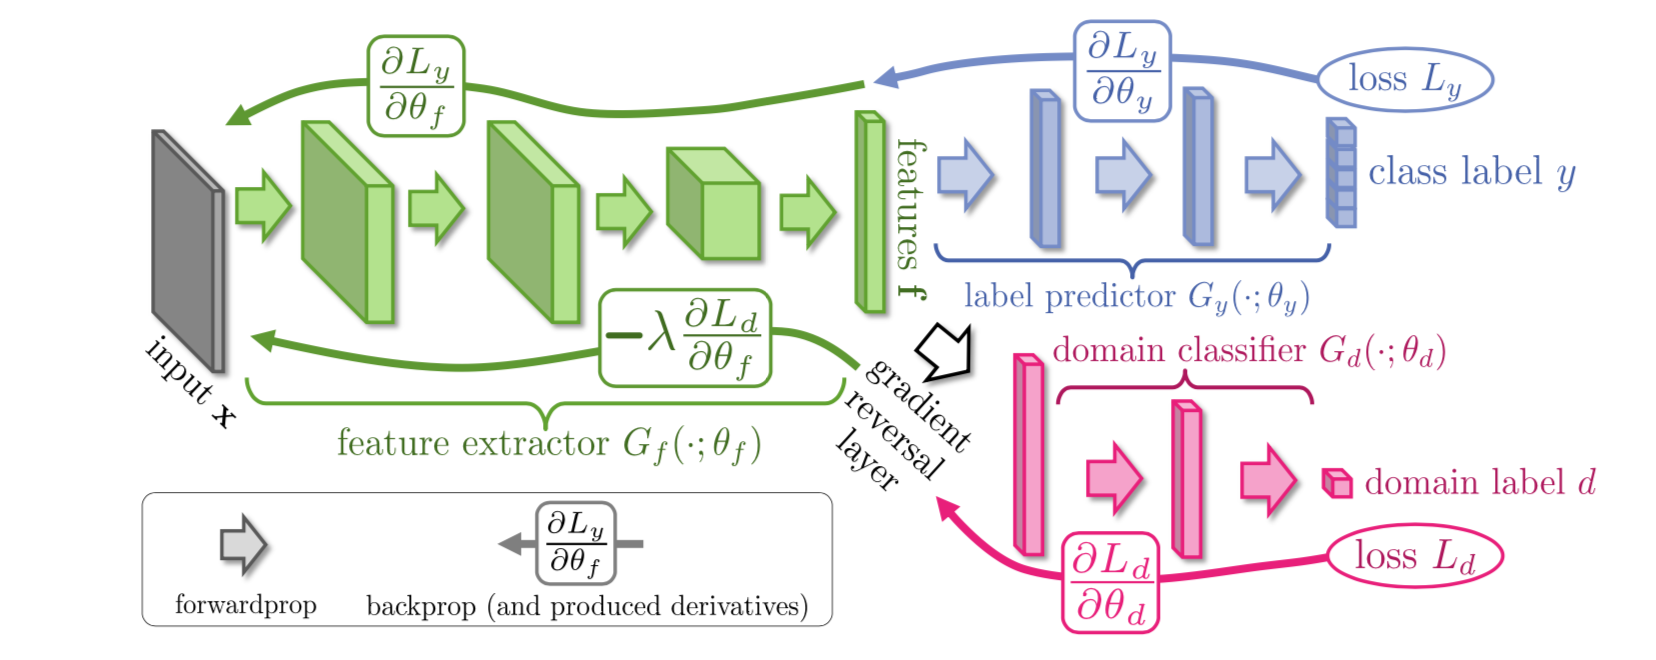
\includegraphics[width=\linewidth]{GRLarch.png}%
    \caption{Architecture with GRL in $G_{d}$ proposed by Ganin and Lempitsky - green part is a \textit{feature extractor} $G_{f}$ that transforms input sample $x$ to feature vector $f$. Afterwards it is classified by \textit{label predictor} $G_{y}$ (blue) and \textit{domain predictor} $G_{d}$ (pink)}
    \label{fig:GRLarch}%
\end{figure}

\section{Research}
\subsection{Paper reproduction}
First stage of all the researches made within the thesis was the paper reproduction. I made all implementations with PyTorch - deep learning python framework developed by Facebook. All computations were run on Google Colab notebook. During most experiments the source domain was MNIST set, while target distribution was MNIST-M. The advanatage of such choice of domains is possibility of quick obtaining a trained model, as architecture needed to classify well MNIST images is not a complex one. Few architectural changes in the network proposed by Ganin and Lempitsky were made, like replacing ReLU activation function with leaky-ReLU and using dropout during training. The accuracy close to the result from paper (81.49\%) was reached after 30 epochs of training, but already after 10 epochs the 77\% of samples from MNIST-M test set were classified well, while accuracy of domain predictor $G_{d}$ was 68\%. Therefore, a long learning process is not needed to verify if the training may be successful.
\par
When I managed to reproduce the paper, the next step was to verify if vector $f=G_{f}(x;\Theta_{f})$ really is domain invariant. When model's parameters were tuned a new domain predictor was constructed, this time without the gradient reversal layer. The input for new classifier was  vector $f = G_{f}(x;\Theta_{f})$ for all samples $x$ from both source and target domain, and the goal was to predict which distribution does $x$ come from. So far we knew that $G_{f}$ mapping was incomprehensible for a single domain predictor $G_{d}$ with parameters $\Theta_{d}$, as it's accuracy was just 68\%, while model that returns always 0 (or always 1) would reach 50\%. If the feature extractor mapping really is domain invariant we should not be able to obtain a model with much better performance.
\par
We could expect that in fact $G_{f}$ mapping is unclear for just one, used during training, domain predictor. After training the new classifier for just 4 epochs, it managed to predict well the domain of 94\% of examples from MNIST and MNIST-M mapped by $G_{f}$. Reaching higher accuracy is just a matter of epochs. Therefore we can certainly say, that representation $f$ of input image $x$ still contains a lot of information about the sample's domain, and getting a real domain-shift invariant representation requires much more than just gradient modification during the training. Nevertheless ability to outsmart a single domain predictor significantly improves the model's performance.

\subsection{Training continuations}
State of the art domain adaptation approaches reach much higher results than a model with GRL. Therefore looking for some improvement is not groundless. With MNIST as source domain and MNIST-M as target distribution, over 90\% accuracy on MNIST-M test set has been reached by most of recent architectures. It should be mentioned that top-performing domain adaptation models apply some data augmentation techniques, which make MNIST more similar to MNIST-M. One of such transformation is adding to the dataset a color-negative version of each sample (white background, black digit). During all my researches no augmentation was made, as in-depth understanding of the DA is more important than results boosting. However, it should be definitely checked if there is any possibility of improving the GRL.
\par
First attempt was based on some mathematical properties. As feature extractor $G_{f}$ maps input to vector $f \in \mathbb{R}^{D}$ we can treat this vector as a point in D-dimensional space. We want representation $f$ of input image not to depend on its domain, that means, we want get to a situation where domain predictor $G_{d}$ requires some feature dependencies that are omitted by $G_{f}$ mapping, so the only features left are useful for the label predictor. Therefore we want $G_{y}$ and $G_{d}$ to use disjoint sets of data dependencies. Transformation made by each of classifier is in fact matrix multiplication. Predictors contain a hidden layer, that maps $f \in \mathbb{R}^{D}$ to some $f_{h} \in \mathbb{R}^{H}$. Moreover, multiplying the coordinates of D-dimensional point, represented by $f$, by some matrix is in fact projecting it onto some directions.  As both models take a point from $\mathbb{R}^{D}$ as an input and process it based on some of its coordinates, we can say, that using disjoint dependencies is in fact transforming the input point with some pairwise (between predictors) orthogonal vectors. Then shifting domain means moving our data along directions that are used by domain predictor, which is unnoticeable for class predictor, therefore representation $f$ remains unchanged, as feature extractor ignore dependencies used by $G_{d}$.
\par
As mentioned before both class and domain predictors have a hidden layer inside. The hidden layer is a matrix $D \times H$ that determines H directions that matters for the model. We can then verify if predictors use orthogonal set of directions by computing the dot product of both matrices. If it is close to zero, the directions are more independent, so more orthogonal. When we compute the mean of square of dot product values after the model's training, it turns out to be a very small number. Therefore directions of $G_{y}$ and $G_{d}$ are almost orthogonal. It may be a good idea to use this learned model and train it again, with modified loss function, that would force $G_{y}$ and $G_{d}$ to minimize that dot product even more. We can add to the objective the mean of square of predictors matrices dot product, i.e. if we denote loss function as $E(\Theta_{f}, \Theta_{y}, \Theta_{d})$ and hidden layer matrices of classifiers as $W_{h_{y}}$ and $W_{h_{d}}$, then new loss function is:
\begin{equation*}
E'(\Theta_{f}, \Theta_{y}, \Theta_{d}) = E(\Theta_{f}, \Theta_{y}, \Theta_{d}) + \overline{(W_{h_{y}} \cdot W_{h_{d}}^{T})^{2}}
\end{equation*}
\par
The new loss function caused reducing of the dot product indeed, but it had no impact on model's performance. As new loss is punishing for product of model's weights the optimizer may force them to decay - lower values implies lower product. This would be undesirable, we want the dot product to reduce not because of shorter vectors, but because of their orthogonality. However monitoring the average length of these vectors shows that they are not shrinking. 
\par
Nonetheless we can add another component to the loss function, that would force $G_{y}$ and $G_{d}$ not only to make their hidden matrices orthogonal, but also to keep column lengths of these matrices unchanged. Once again, even the new loss function meets the expectations, model's performance doesn't improve.
\par
I decided to check if preventing the decay of these matrices weights is necessary, so instead of punishing for shrinking, the model was forced to to minimize the dot product of $W_{h_{y}}$ and $W_{h_{d}}$ as much as possible. When only the new loss with weight regularization was applied, the values quickly got close to zero. However it did not make the model performance worse, the accuracy over the epochs get even more stable. This experiment shows also, that weight decay usually is a good optimization practice.
\par
Extending the loss function in order to increase orthogonality of directions used by label and domain classifiers did not improve the model's performance. We could notice that before adding new components to loss function, these directions already were almost orthogonal, as GRL's task is to force the predictors to use disjoint features of their common input. As mathematical approaches did not enhance the network's result, some different attempt to improve the model should be done.
\subsection{Training continuation with increased $\lambda$}
The $\lambda$ coefficient grows from 0 to 1, as the feature extractor's output should be firstly adjusted to label predictor, and then made more and more domain invariant. When the final model is obtained, parameters $\Theta_{y}$ are well tuned, as accuracy on source domain - MNIST test set is about 99\%. $G_{y}$ is already well trained then, the only limitation is not domain invariant enough transformation made by $G_{f}$. As forcing this invariance is the $G_{d}$ aim, we could try to increase its impact on $G_{f}$ when $G_{y}$ is well trained. Therefore the new continuation of the learning process has a single modification - $\lambda$ has fixed value, that is greater than 1. In first attempt $\lambda$ was set to 3. After 10 epochs the model had 79.2\% accuracy on MNIST-M test set, for next 10 epochs of training fixed $\lambda$ was used, and the result increased to 80.8\%. If we train a fresh model for 20 epochs with increasing $\lambda$, we would reach comparable accuracy, so we cannot be sure, that the continued training with higher and fixed $\lambda$ will often improve the model's performance. However it seems reasonable to apply this kind of continuation, when larger epochs number does not help.
\par
Setting $\lambda$ parameter to some value grater then 1 is enhancing the impact of domain predictor on feature extractor mapping. However if the coefficient would be too large, it may lead to a decrease of label classifier accuracy. During experiments, when $\lambda = 6$ a pre-trained model gets chaotic, its result fluctuate over the epochs, and does not reach the level from first training. Therefore we should worry about picking the right value for $\lambda$ coefficient during training continuation.

\subsection{Adding GRL to well performing domain predictor}
As verified before, feature extractor produces representation that is indistinguishable for a single domain predictor. After the training we can easily obtain a model that successfully predicts the distribution of the sample, if only its architecture does not contain the GRL. We can check then, how difficult and effective would be changing the transformation made by $G_{f}$, so it become unclear for the well performing domain predictor, denoted as $G_{d}'$. We add the gradient reversal layer at the begining of the classifier's architecture. Then we train the whole model once again, but now the components are $G_{f}$, $G_{y}$ and $G_{d}'$. 
\par
After just few epochs accuracy of $G_{d}'$ has decreased significantly, as $G_{f}$ mapping adjusted to the new architecture. However, classifying samples from target distribution has not got any better. Also we don't know, how the $G_{d}'$ with GRL differs from $G_{d}$. If in fact both these predictors use highly correlated features to compute their results, then they are almost equal. Moreover, during training the whole model with $G_{d}'$, we don't use $G_{d}$ anymore, so we can't say, that $G_{f}$ produces the representation that is unclear for two domain predictors. Maintaining multiple domain classifiers may cause some improvement, however this approach would explain neither how GRL helps in DA task, nor what really is domain adaptation. Therefore it was not implemented.

\subsection{Adam Optimizer}
Stochastic gradinet descent (SGD) is probably the most popular optimizer used in deep learning. However, in recent years some fancy optimization methods released and they can boost the training process even more. One of them is Adam Optimizer. It is much more complex than SGD, with individual learning rate for each parameter and usage of more gradient properties. 
\par
To check if Adam may improve our model, the optimizer for each network was changed. After 10 epochs of training accuracy on target domain was slightly higher than before. The dot product of predictors hidden layers matrices was much higher than in the SGD case, therefore once again the modified loss function was used to minimize the dot product. The modification caused quick decay of this value, however the target domain performance did not change. Anyway, Adam optimizer turned out to be a good choice. Its parameters should be initialized carefully, as during the training the loss may get NaN value much easier. In our particular case, the initial learning rate was reduced from 0.01 for SGD to 0.001 for Adam.

\subsection{Tuning model size}
So far we did not manage to force the network to separate the information about the domain from some digit features. $G_{f}$ mapping satisfies both label and domain predictor, as we can easily obtain a successful domain classifier, so the representation $f=G_{f}(x;\Theta_{f})$ of input sample $x$ is not domain shift invariant. During all previous experiments, feature vector $f$ was 320-dimensional. Maybe the size is so large, that $G_{y}$ uses only its fraction, and the rest of the space is filled with information about the distribution of the input. Therefore a decreasing of $G_{f}$ output size should be considered.
\par
The intuition is that maybe there is an optimal size of feature extractor output. It would be big enough for $G_{y}$ to predict input's label with as high accuracy as with current architecture, but space left unused by class predictor would be too little to be sufficient for any domain predictor. The approach with a domain classifier without GRL should also be tried. If two models would compete for space of feature vector $f$, if it was too small, one of the network would "lose" and had no opportunity to learn.
\par
So far feature extractor was constructed with only convolution layers. During these experiments it was extended by single fully connected layer that was mapping the last convolutional layer's output from $\mathbb{R}^{320}$ to $\mathbb{R}^{D'}$, where $D' = 280, 240, 200, 180, 160, 120$. Then the smaller feature vector was classified by class predictor $G_{y}$ and domain predictor $G_{d}$ containing GRL. 
\par
When feature extractor tries to store all the features in lower dimension, the training process gets noisy. If the number of dimensions $D'$ is too little, value of the loss function may become NaN. It happens if the training lasts for too little epochs, when $\lambda$ gets close to 1 quickly and feature extractor is confused with two different gradients from $G_{y}$ and $G_{d}$. As $G_{f}$ returns just few values, both predictors compete for significant changes in most of them, what lead to the failure of the training. GRL may handicap the learning process then.
\par
After training each architecture the results were not surprising at all. The more complex the model was, the higher accuracy it reached. Moreover, adding fully connected layer caused noticeable fall of performance.  Figure~\ref{fig:size_tune} presents the accuracy of each model. 
\begin{figure}[htb]%
    \centering
    \includegraphics[width=\linewidth]{size_tune.png}%
    \caption{Accuracy of models with different feature extractor output size over the epochs. The \textbf{model 0} is the architecture used during previous experiments, with 320-dimensional $G_{f}$ output. \textbf{model 1 - model 6} are build with feature extractor that is extended with single fully connected layer, which return feature vector in smaller dimension, respectively: 280, 240, 200, 180, 160, 120. Labels present results on MNIST-M test set. We can see, that adding a fully connected layer caused decreasing of model's accuracy. }
    \label{fig:size_tune}%
\end{figure}

\par
As two different models use the feature extractor's output, $G_{f}$ tries to produce the result that would fit for both classifiers. So far GRL was jumbling it with purpose to make $G_{f}$ output clear for label predictor and as impenetrable as possible for domain classifier. If $G_{d}$ doesn't contain a gradient reversal layer, it would act like a regular binary classifier. The feature extractor would then try to return an output that would contain information about both the label of the input, as well as the domain of the sample. Therefore if the $G_{f}$ output would be too small, one of the classifier could receive too little data to learn well. If it would be the domain predictor, then the representation gets domain invariant.
\par
Once again feature extractor is extended by fully connected layer. This time it maps the feature vector to even 5-dimensional space. Our goal now is to train $G_{y}$ and $G_{d}$ to reach high accuracy simultaneously. When all the models are learned resluts are unsatisfactory. In each case both label and domain predictor perform well within their tasks - $G_{y}$ reaches over 98\% accuracy on MNIST test set, even when feature vector $f$ is 5-dimensional. Domain classifier in every architecture is almost always right. However there is an enormous decrease in target domain classifying performance - all the models have accuracy on MNIST-M test set under 20\%, twice less than a simple CNN trained on MNIST.
\par
Such a poor result definitely is a disappointment. Not only all the intuitions were wrong - limiting the output space did not force feature extractor to separate the data, but even model's performance get much worse. It seems that domain predictor's impact on feature extractor is so high, that the $G_{f}$ mapping becomes highly correlated with the distribution of the input, therefore, when we transform sample from target domain its representation is meaningless. Straightforward using of common feature vector mapping for two architectures is not a good idea then.

\subsection{Domain information vanishing}
Absence of domain information in feature vector is highly desirable in domain adaptation problem. Unfortunately GRL does not force such representation, as distribution predictor can be easily obtained - with 16 epochs of training the model achieved 95\% accuracy. Therefore, label classifier prediction is dependent on domain of the input image. Checking how successful can be a domain classifier on class predictor's first layer would show the magnitude of this dependency. 
\par
After 16 epochs of such classifier's training its accuracy in prediction the distribution of the input image was 88\%, then a decay of domain information happened, which improved the performance on target domain. Therefore, the growth of uncertainty of distribution classifier may cause even better results. This leads to the next experiment - "plugging" a domain predictor with GRL to the output of the first layer of class predictor. The weights of feature extractor are frozen now, as we don't want to change its mapping. The task now is to take the transformation, that leaves 88\% of information about the distribution of the input, and try to decrease this result with GRL.
\par
When the new domain classifier was applied to the output of $G_{y}$ first layer, after 16 epochs of training the accuracy on target domain test set was slightly better. To check if the distribution information had vanished even more, the new domain predictor was learned. Its accuaracy reached 75\%, therefore applying GRL to the output of the layer had definitely made in more domain invariant. This observation induces to check if the decay of distribution information would advance in deeper layers of the architecture.
\par
A special architecture of the network was used during thus experiment. Class predictor so far was built with an input layer, a single hidden layer and the output one. This time it was extended with an extra hidden layer. With deeper model we can monitor more precisely the decay of domain information. 
\par
After 16 epoch of training the accuracy of the model on the target domain (MINST-M) test set was 78.6\%. Then the feature extractor was frozen and the new distribution classifier (without GRL) was obtained to measure the domain information in $G_{f}$ output. Afterwards the first layer of $G_{y}$ was used just like feature extractor. The new $G_{d}$ with GRL was plugged to its output, therefore, the layer's mapping was used by the rest of class predictor and the domain classifier as well. This should lead to making the layer's output more domain invariant, what was checked with obtaining next distribution predictor. The procedure was then repeated on following layers of $G_{y}$. Table~\ref{tab:domain_vanishing} shows the results of predictors on each stage. Measuring domain information or applying model with GRL on $G_{y}$ output layer would be pointless, as these values are probabilities of each digit. Figure~\ref{fig:domain_v} presents the described learning process.

\begin{table}
\begin{center}
\begin{adjustbox}{width=1.2\textwidth,center=\textwidth}
\begin{tabular}{c|c|c|c|c}
\multicolumn{1}{l}{} & \multicolumn{1}{l}{} & \multicolumn{1}{l}{} & \multicolumn{1}{l}{} & \\
Accuracy of \textbackslash{} model's layer & $G_{f}$ output  & input & ~1st hidden & 2nd hidden \\ 
\hline
Domain classifier on output & 99.99\%~ & 87.86\% & 75.13\% & 69.47\% \\ 
\hline
Domain classifier after adding GRL~ & 95.95\% & 74.75\% & 68.19\% & 68.6\%  \\ 
\hline
\begin{tabular}[c]{@{}c@{}}Target domain test set classification \\(after applying domain predictor with GRL)\end{tabular} & 78.6\% & 78.74\% & 79.06\% & 79.26\%    
\end{tabular}
\end{adjustbox}
\caption{Domain information vanishing research - for output layer of $G_{f}$ and input and both hidden layers of $G_{y}$ firstly the best possible domain predictor is obtained, then the $G_{d}$ with GRL is applied to the layer and accuracy of classifying the target domain test set and sample distribution are measured. While plugging model with GRL to one of the $G_{y}$ layers, the feature extractor and all previous layers of $G_{y}$ are frozen}
\label{tab:domain_vanishing}
\end{center}
\end{table}

\begin{figure}
    \centering
    \vspace*{-3cm}
    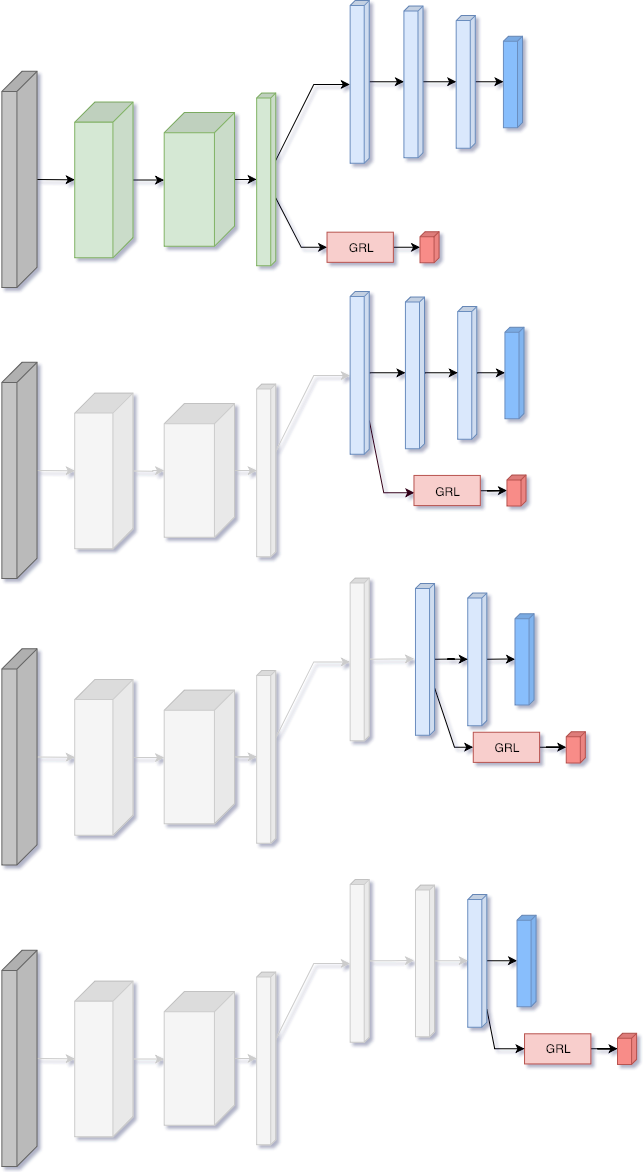
\includegraphics[scale=0.45]{domain_v.png}%
    \caption{Domain information vanishing process. Firstly the domain predictor is plugged to the output of $G_{f}$. Then $G_{f}$ is frozen and model with GRL is applied to the input layer of class predictor. In consecutive stages the layer is frozen, and GRL is plugged to the following one. Green blocks represent $G_{f}$, blue ones $G_{y}$ while pink are domain predictor $G_{d}$. Grey blocks are frozen layers. Best viewed in color.}
    \label{fig:domain_v}%    
\end{figure}

\par
Adding a domain predictor with GRL definitely caused the decay of distribution information, as applying it on $G_{y}$ input layer decreased the accuracy of domain classifier by 15\%. Therefore, the information passed by the first layer of class predictor is not as disturbed by distribution features as before. The experiment shows that applying model with GRL to layers of label classifier makes it more domain invariant. However, performance on test set from target distribution did not improve significantly, basic model with single domain predictor reaches similar result. Nonetheless it seems to be a good practise to apply GRL to more layers.
\par
Vanishing of domain information in deeper layers may be also caused by the complexity of input image transformation on this stage. The small decrease of domain predictor accuracy confirms the small impact of adding model with GRL. It seems like applying an extra domain classifier is more reasonable on early layers of $G_{y}$. It may be helpful observation, if the learning process lasts for a long time. 
\par
The deeper model was not as accurate as the one with single hidden layer in class predictor. Therefore, the experiment was repeated on the smaller model. Each stage of the learning process lasted 16 epochs Plugging the domain classifier to the layer's of this model also caused the decay of distribution information and an improvement on MNIST-M test set. Finally the model reached 80.7\% accuracy on it, while basic model trained for same number of epochs couldn't get higher than 80.57\%. Table~\ref{tab:domain_v_single_hidden} presents detailed results.
\begin{table}
\centering
\begin{tabular}{c|c|c|c}
\multicolumn{1}{l}{} & \multicolumn{1}{l}{} & \multicolumn{1}{l}{} & \\
Accuracy of \textbackslash{} model's layer & $G_{f}$ output & input & ~hidden \\ 
\hline
Domain classifier on output & 99.99\%~ & 89.69\% & 77.43\%  \\ 
\hline
Domain classifier after adding GRL~ & 93.95\% & 78.28\% & 71.83\%  \\ 
\hline
\begin{tabular}[c]{@{}l@{}}Target domain test set classification \\(after applying domain predictor with GRL)\end{tabular} & 76.91\% & 80.6\% & 80.7\%  
\end{tabular}
\caption{Domain vanishing for a model with single hidden layer.}
\label{tab:domain_v_single_hidden}
\end{table}
\par
Applying a new domain predictor with a gradient reversal layer turned out to be a successful modification. Although the improvement of results was small, the inner representations of input data are definitely more domain invariant, therefore it might be crucial in some situations. Also it came out, that if computational cost of applying new classifier to each layer is too high, the best practise is to use it with first layers of the label predictor.

\subsection{SVHN experiments}
All foregoing experiments were made when the source and target domains were MNIST and MNIST-M. Very high degree of relatedness between them may  be worrying, therefore the experiments made so far should be verified with some other datasets. One of the others digit image collections is the mentioned previously Street View House Numbers (SVHN) dataset. It was used as source domain, so the label classifier was learned with its samples. MNIST was a target distribution this time.
\par
SVHN is much more complex dataset, with many fuzzy images that presents more than one digit. Therefore obtaining well-performing model requires not only the longer training, but also more advanced architecture. The one used in following experiments had a feature extractor built with 5 convolutional layers, each one using batch normalization and the leaky-ReLU followed by max pooling and dropout during training process. The class and domian predictors have larger hidden layers than before. This architecture allows us to get reasonable results after about 18 epochs. The model proposed by Ganin and Lempitsky was not that complex, but they trained it for much longer, as for first 150 epochs classification error was high during their research.
\par
First training was a basic reproduction of GRL usage. The obtained model classified well 93\% of samples from SVHN test set and 76.5\% images from MNIST test set, slightly higher than best model obtained by the authors (71.07\%). Afterwards, the model built with just a feature extractor and class predictor was learned. The accuracy on SVHN test set was 94\% this time. Despite absence of a domain predictor with GRL, the model managed to recognize well 68\% of MNIST images. Such a well performance on target domain (Ganin and Lempitsky reached 59.19\%) is the result of the complex architecture.
\par
Just like in previous case, domain information is still available after $G_{f}$ mapping, we can easily get almost perfect distribution predictor. Also modifying the loss function with some mathematical theories did not improve the target domain performance. Applying the domain classifier with GRL succeed in partly removing the distribution information from $G_{y}$ layers, but did not increase the model accuracy on MNIST test set this time. Using Adam as optimization algorithm caused an improvement - not only the training was more stable, but the accuracy on target domain test set was 75\%.
\par
Repeating all the experiments with SVHN and MNIST as domains shows, that strong correlation between MNIST and MNIST-M was not the only reason of GRL partial success in domain adaptation. The improvement of the performance beside the model without domain predictor is then really caused by the ability of the network to focus on the semantic of the image - a digit. Obtaining domain-shift invariant representation of the input data does not happened with just GRL, but definitely such transformation would bring a huge triumph in DA.

\section{Gradient modifications}
Gradient reversal layer is nothing but a simple modification of the gradient. Executed experiments show, that multiplying the gradient by some negative value brings a great improvement in the domain adaptation. The motivation of GRL is producing the domain invariant representation, by following during backpropagation the opposite direction of the domain predictor's gradient. Despite the reality is significantly different, the results are satisfying. Therefore it should be verified, how important for the improvement is transforming the gradient in that particular way, and what is the result of some other modifications.

\subsection{Random gradient replacement}
First of tested gradient modifications is replacing the real gradient with some random numbers. Formally, if $Rand()$ is a function returning the random real number from range $(0,1)$, replacing the gradient is:
\begin{equation*}
GradRand_{\alpha}(x, \lambda) = \begin{cases}
x &\text{forward pass}\\
Rand() \cdot \alpha \cdot \lambda &\text{backward pass}
\end{cases}
\end{equation*}
\par
The function is parameterized by $\alpha$ that is scaling the range of random number. Simultaneously multiplying by $\lambda$ is kept, as it is still increasing over the training, to enhance the impact of gradient modification. One could say, that both $\alpha$ and $\lambda$ don't matter as multiplying a random value by some scalar results in a random value, but limiting its range is crucial to avoid training failure.
\par
Used architecture was again built with feature extractor $G_{f}$, label predictor $G_{y}$ and domain classifier $G_{d}$. The only difference is that first layer of $G_{d}$ was a gradient random layer, which was performing $GradRand_{\alpha}$ function. Initially the $\alpha$ was set to 1. After few epochs of training, when $\lambda$ increased above small value, the loss function of the model became NaN. When $\alpha$ was decreased to 0.1 and 0.01, the failure of training repeated. It was needed to use $\alpha = \frac{1}{1000}$ to end up with successful training.
\par
Such a low value of $\alpha$ causes the lack of $G_{d}$ impact on feature extractor. $G_{f}$ was tuning its parameters basing on $G_{y}$ gradient and a little noise from domain predictor, as its gradient was a value from range $(0, \frac{1}{1000})$. Moreover the real gradient of domain classifier is ignored at all, therefore it could not be computed as well. Therefore the results of the model are not surprising - classification of examples from both source domain, which was again MNIST and MNIST-M, was as good as in model without any extra domain predictor. The $G_{d}$ reached very high accuracy in domain predicting, as there was nothing that would disturb it.
\par
Replacing gradient by some random does not seem very effective. Firstly, the random value must be small, otherwise, the training fails. Secondly there was not any improvement of the model. Moreover tuning parameters of $G_{d}$ was an unnecessary computational effort. Nevertheless adding some random values to the real gradient may be considered as an attempt to avoid overfitting, as it may slightly decrease the impact of real data.

\subsubsection{Random gradient multiplying}
Second attempt to modifying the gradient of domain predictor was also based on random values. This time instead of simple replacement, the real gradient was multiplied by some random number. Once again its range was parameterized by $\alpha$ coefficient. The increasing $\lambda$ was also used over training epochs. The modification may be specified as:
\begin{equation*}
GradRandMult_{\alpha}(x, \lambda) = \begin{cases}
x &\text{forward pass}\\
Rand() \cdot \alpha \cdot \lambda \cdot x &\text{backward pass}
\end{cases}
\end{equation*}
\par
The architecture of learned model was changed, so domain predictor was performing $GradRandMult_{\alpha}$ at the beginning. This time using $\alpha = 1$ did not cause the failure of training, but the model's behaviour was simmilar to the situation, when both $G_{y}$ and domain predictor $G_{d}$ without GRL were influencing the feature extractor. Model was effective on source domain test set and managed to predict the distribution of the input, but accuracy on target domain was terrible, just 28\% on the MNIST-M test set. This seems reasonable, as the gradient is now multiplied by some value from range $(0,1)$, while in the case without random number it was always 1. Therefore the bad impact of the domain predictor was slightly lower and the result on target domain is then a bit better, but very unsatisfying.
\par
Afterwards the $\alpha$ was set to 0.1, what considerably improved the previous model. While domain predictor's performance and accuracy on source domain test set kept over 99\%, the result on target distribution increased to 50\%. These results are similar to the score of model without domain classifier. As the impact of $G_{d}$ on feature extractor is rather low, this behaviour could be expected.
\par
Some bigger changes in model's performance could have been noticed if the $\alpha$ parameter was set to a negative value. The model behaved then similarly to the architecture with GRL. If $\alpha = -\frac{1}{10}$ accuracy on MNIST test set kept 99\%, while target domain samples were recognized correctly in 67\%. Moreover the accuracy of $G_{d}$ fell to 81\%. These results shows that the gradient multiplication with such $\alpha$ behaved just like a soft version of GRL.
\par
Afterwards $\alpha$ was set to -1, so the gradient was scaled by negative number from range $(-1, 0)$. As it could have been expected the result was close to the performance of model with GRL - MNIST test set was classified well in 99\%, accuracy on MNIST-M was 76\% and $G_{d}$ result was down to 72\%. The model performed just like it was using GRL, and it seems reasonable.

\subsection{Gradient inversion layer}
The reversion of the gradient's direction points at the function maximum. Therefore, the intuition behind GRL is to find such parameters $\Theta_{f}$ of feature extractor, that the domain predictor $G_{d}$ is as incorrect as possible. These parameters can be found if $G_{f}$ tunes them w.r.t. the reversion of $G_{d}$ loss function gradient's direction.
\par
The gradient not only points the direction of function's minimum, but also determines the magnitude of each parameter's impact on final result, as gradient is a multi-variable derivative. Therefore, when the goal is to set such parameters $\Theta_{f}$, that transformation made by $G_{f}$ is absolutely meaningless for domain predictor, reversing the magnitude of gradient's value should be considered. It would cause that crucial changes for $G_{d}$ would be ignored, while parameters that were already well tuned from domain predictor point of view, would be significantly changed. Moreover each value would had its sign changed, so the direction opposite to the one pointing at minimum would be followed. 
\par
Such modification could not only force feature extractor to tune its parameters in a way that loss function of $G_{d}$ gets higher and higher value, but also to disallow the domain predictor from finding any dependencies. If only $G_{d}$ finds pattern in some $G_{f}$ parameters they are changed much more than some irrelevant ones, so no meaningful information about domain would occur in feature extractor mapping. 
\par
The described transformation could be specified as function, which argument is a vector of real values $x = [x_{0}...x_{D-1}]$. Once again during forward pass it remains unchanged, while the modification is made during backpropagation:
\begin{equation*}
GradInverse(x, \lambda) = \begin{cases}
x &\text{forward pass}\\
-\lambda \cdot (\max_{0 \leq i < D} |x_{i}| \dotdiv x) &\text{backward pass}
\end{cases}
\end{equation*}
where $\dotdiv$ is element-wise difference - for each value of the vector $x$ it is subtracted from the largest absolute value from the entire vector.
\par
Such transformation can be inserted at the beginning of the model just like GRL. The computational cost of the training is a bit bigger, as for each input sample the maximum value must be computed. Nevertheless, learning MNIST classification does not take a long time.
\par
Results of the model with domain predictor $G_{d}$ started with $GradInverse$ are promising. 
After just 10 epochs of training the accuracy on MNIST-M test set was 78.87\%. A model with GRL instead of $GradInverse$ managed to get just a bit better result. Moreover, the domain predictor $G_{d}$ classified well only 58\% of all samples, which is much lower than when GRL was used.
\par
Using $GradInverse$ was supposed to decrease the score of the domain classifier by tuning the feature extractor parameters absolutely opposite to its requests. With no doubt model with $GradInverse$ succeed in this task. The accuracy of classifying examples from target domain was a bit lower than with GRL, but inversing the magnitude of the gradient's absolute values definitely is a new option in domain adaptation. The partial success of this approach shows also, that some other gradient modification may cause even better performance than GRL.

\section{Conceptors}
\subsection{Domain adaptation as point cloud transformation}
Although some of the experiments gave interesting results, none of them improved significantly the GRL approach. Unquestionably, domain adaptation is a very complex problem, therefore understanding it could be crucial to find some better solutions. As previously mentioned the representation of input sample $x$ after mapping by feature extractor $G_{f}$ is a feature vector $f = G_{f}(x ; \Theta_{f}) \in \mathbb{R}^{D}$. It may be also considered as a point in $\mathbb{R}^{D}$. All the samples from source domain $S$ and target domain $T$ form a point clouds in $\mathbb{R}^{D}$ space that can be denoted as $F_{S}$ and $F_{T}$ respectively:
\begin{align*}
    F_{S} &= \{ G_{f}(x_{s} ; \Theta_{f}) : x_{s} \in S  \} \\
    F_{T} &= \{ G_{f}(x_{t} ; \Theta_{f}) : x_{t} \in T  \}
\end{align*}
\par
If the transformed samples from both domain are considered as points, the feature extractor should find a mapping, that produces as similar point clouds form distributions as possible. Then, the domain classifier could not predict well, if point form $\mathbb{R}^{D}$ with given coordinates belongs to either point cloud $F_{S}$ or $F_{T}$. Obtaining such representation would be a half way to success, as perfect mapping should also place the samples from a single class in the same region for both domains. The label predictor $G_{y}$ would then have to just find a division of the space into the regions for all classes.
\par
If the source domian is MNIST and the target distribution is MNIST-M then the input image, that has resolution $28\times28\times3$, is a point in $28\cdot28\cdot3 = 2352$ dimensional space. If a feature extractor $G_{f}$ maps it to a 320-dimensional feature vector, then the transformation made by $G_{f}$ may be seen as a function $\mathbb{R}^{2352} \rightarrow \mathbb{R}^{320}$. The obtained point clouds may be denoted as $F_{MNIST}$ and $F_{MNIST-M}$.
\subsection{Conceptors}
It is not a simple task to find a description of points cloud in $\mathbb{R}^{D}$ that would be understandable for a human, if $D = 320$. Nevertheless, it is possible to approximate these points somehow. One approach is to find an ellipsoid in $\mathbb{R}^{D}$ that captures the majority of the points. This idea was used by Herbert Jaeger to introduce the concpetors. Such ellipsoid is then used to transform a new point into the cloud of known points. The conceptor is defined as a matrix $C$ that determines an ellipsoid that approximates a given point cloud and is then normalized, so it lies inside the unit sphere. Figure~\ref{fig:conceptor_intro} presents a simple visualization of this idea.
\begin{figure}%
    \centering
    \includegraphics[width=\linewidth]{c_example.png}%
    \caption{Point clouds (black) and conceptors approximating them. Best viewed in color.}
    \label{fig:conceptor_intro}%
\end{figure}
Singular vectors of matrix $C$ are the principal axes of the described ellipsoid, while singular values of $C$ are their lengths. They can be easily obtained with SVD method. The conceptor matrix $C$ is obtained with correlation matrix $R = \mathbb{E}_{x}[xx^{T}] \in \mathbb{R}^{N\times N}$ of samples $x \in \mathbb{R}^{N}$ and the aperture parameter $\alpha$, as:
\begin{equation*}
    C = R(R + \alpha^{-2} I)^{-1}
\end{equation*}
\par
The transformation of given point $x$ into the conceptor is made by multiplying it by the matrix $C$. If $x$ lies inside the ellipsoid that is described by the conceptor, the multiplication should act like identity and remain $x$ unchanged. If $x$ is a point from the outside of the ellipsoid then $C$ should move it inside. This idea sounds attractive for domain adaptation. Firstly the point clouds $F_{S}$ and $F_{T}$ could be approximate by ellipsoid and corresponding conceptors could be computed. Measuring the similarity of $F_{S}$ and $F_{T}$ would be just conceptors comparison. Moreover, the concpetor matrix multiplication could be a new domain adaptation approach. After computing the conceptor $C_{S}$ for data cloud $F_{S}$, while input sample $x$ would be classified, its feature vector $f = G_{f}(x ; \Theta_{f})$ could be multiplied by $C_{S}$ before processing by $G_{y}$. This would transform it into data cloud that is already well known for the label predictor. Therefore the probabilities for each class would be computed as:
\begin{equation*}
  P(x) =  G_{y}( G_{f}( x ; \Theta_{f} ) \cdot C_{S} ; \Theta_{y} )    
\end{equation*}
\par
As conceptor always lies inside an unit sphere, it can be measured, how much of space does it occupies. If the point cloud that is approximated with a concpetor is scattered over the whole space then it would not be possible to approximate it with nothing but a sphere. However, if points are located in an organized cluster, they can be captured with much more limited ellipsoid. Therefore, the \textit{quota} value measures the fraction of the space that is taken by a conceptor. It can be computed as:
\begin{equation*}
    Q(C) = \frac{1}{N} \sum_{i=1}^{N}{s_{i}}
\end{equation*}
where $s_{i}$ are singular values of conceptor matrix $C$. Moreover, logic operations  can be applied to the conceptors, such as $\neg, \vee, \wedge$. The negation of conceptor is the space orthogonal to the ellipsoid, the disjunction is a conceptor that is obtained with sum of samples sets, while the conjunction is the conceptor that approximates the intersection of these sets. Figure~\ref{fig:conceptor_logic} charts these operations.
\begin{figure}%
    \centering
    \includegraphics[width=\linewidth]{c_logic.png}%
    \caption{Logic operations on 2-dimensional conceptors.}
    \label{fig:conceptor_logic}%
\end{figure}
\par
\subsection{Point clouds similarity with conceptors}
To assess the similarity of two point clouds corresponding conceptors $C_{S}$ and $C_{T}$ should be computed firstly. Then $C_{S} \vee C_{T}$ is their intersection. The value $Q(C_{S} \vee C_{T})$ determines its magnitude. If it is close to both $Q(C_{S})$ and $Q(C_{T})$ then ellipsoids that approximate both point clouds are similar. The quota of conjunction $Q(C_{S} \wedge C_{T})$ should also be close to the $Q(C_{S} \vee C_{T})$, as intersection of these point clouds should include most of them.
\par
Reliable result demands well computed conceptors. The final values of matrix $C$ depend on the magnitude of the scaling parameter $\alpha$, called the aperture. If it is too low, the conceptor acts as zero mapping, while when the aperture is getting larger, the conceptor matrix becomes an identity matrix, therefore, finding the right aperture is crucial. Jaeger propose some methods for analytical finding the right value of $\alpha$ for an echo-state network, which can be used if needed.
\par
Described approach was used to measure the similarity of $F_{S}$ and $F_{T}$ point clouds. The domains were MNIST and MNIST-M, and feature extractor $G_{f}$ was mapping an input image to 320-dimensional feature vector $f$, so the conceptor matrices were $C_{MNIST} \in \mathbb{R}^{320}$ and $C_{MNIST-M} \in \mathbb{R}^{320}$. Computational cost of obtaining these matrices is low, even for 60000 samples from dataset, therefore many different setups may be tested.
\par
Xu He and Herbert Jaeger published the paper "Overcoming Catastrophic Interference using Conceptor-Aided Backpropagation", where conceptors are used to enable a neural network to learn MNIST and its permutations. Their goal is to obtain a model, that is already trained for some tasks and make it perform well on another one, without an accuracy deacrease for previously learned problems. The first domain for their network is MNIST, while each of following datasets is the MNIST with a random permutation of pixels applied for all samples. All the distributions are equally difficult to classify as the original MNIST. During the learning process the $A$ conceptor is describing the space already taken, so the next task tries to use only its complement $\neg A$. At the beginning of the training, the authors compute the conceptor $C_{0}$ for the MNIST dataset, and they train the model. The $A$ is equal $C_{0}$ then. During $i-th$ task the conceptor $C_i$ for training samples is comupted, and the model tries to transform it into $F = \neg A$. If it succeed, the conceptor $W_{i}$ is the space used by the $i-th$ task, and the $A$ is updated: $A = A \vee W_{i}$. The $Q(A)$ value is monitored during the training, as it determines the ability to learn a new task by the model. When $Q(A)$ gets 1 there is no spare space, and trying to fit any other dataset fails. 
\par
As Xu He and Jaeger use MNIST as their main dataset and receive some satisfying results it seems reasonable to use the same aperture $\alpha$ as the authors. For most of experiments in their paper, the $\alpha$ was set to 4. When such value was used to compute the $C_{MNIST}$ and $C_{MNIST-M}$ conceptors, their quota values were both over $0.99$. This was highly undesirable, as it implied that the points form both point clouds were scattered over the space, therefore the ellipsoids approximating them were not a good depiction. Even the value $Q(C_{MNIST} \vee C_{MNIST-M} )$ and $Q(C_{MNIST} \wedge C_{MNIST-M} )$ were close to each other and to quotas of each conceptors, it did not mean the $F_{MNIST}$ and $F_{MNIST_M}$ were similar. We could only conclude that points from these cloud lied in many regions of the space. 
\par
The lower value of $\alpha$ was used, but for any $\alpha > 1$ the quota of conceptor was over $0.99$, to obtain $Q(C_{MNIST}) < 0.9$ it was needed to set $\alpha = 0.4$. With such low aperture it is hard to say if the results are reliable, as in all experiments made by Xu He and Jaeger, the $\alpha$ was much larger. However, for all tested values, the $Q(C_{MNIST})$ and $Q(C_{MNIST-M})$ were close.
\par
The only interesting result was obtained when the model was trained without the domain predictor $G_{d}$. When the parameters of the model depended only on MNIST samples, the $Q(C_{MNIST})$ was as high as in previously described case, for any $\alpha > 1$ it was over $0.99$. However when $C_{MNIST_M}$ was computed, the quota of the conceptor was clearly lower. As $F_{MNIST-M}$ may be captured with a smaller ellipsoid, then it must be different from $F_{MNIST}$, so classification the MNIST-M samples is much less accurate. Figure~\ref{fig:Q(C)} presents the quota values of $C_{MNIST}$ and $C_{MNIST_M}$ when aperture was in range $[0.1, 1]$.

\begin{figure}
    \centering
    \subfloat[Model trained with GRL]{{\includegraphics[width=5.5cm]{Q(C).png} }}%
    \qquad
    \subfloat[Model trained without GRL]{{\includegraphics[width=5.5cm]{Q(C_nogrl).png} }}%
    \caption{Quota of concpetors $C_{MNIST}$ (blue) and $C_{MNIST_M}$ (green) for training with or without domain predictor with GRL.}%
    \label{fig:Q(C)}%
\end{figure}

\section{Visualization}
\par
To get some intuitions about how Gradient Reversal Layer and Conceptors work I tried to visualize the output of feature extractor. To do so I added an extra layer $G_{3}$ that takes from feature extractor $G_{f}$ the output vector ${ f } \in { R } ^ { D }$ and maps it to ${f'} \in {R}^{3}$, so the input vector ${x}$ is mapped into 3-dimensional space as $G_{3}(G_{f}(x))$. Now we can treat it as a 3-dimensional point. 

\subsection{MNIST and MNIST-M}
\par
Training model with such a small layer inside is much more difficult task, as many information may be lost during mapping do ${R}^{3}$. Therefore at the beginning I tried to get a simple MNIST classifier with no Gradient Reversal Layer. Fortunately the model achieved 98\% accuracy on the test set, but it performed poorly on MNIST-M - it managed to recognize just 31\% of digits, while without 3D mapping model's accuracy is 61\%. Now we can check how the input space ${X}$ looks after mapping by feature extractor. Figure~\ref{fig:MNIST_3D}(a) shows the result of mapping for all samples from MNIST test set (blue) and MNIST-M test set (gray). Each point represents coordinates of vector obtained by passing it through feature extractor with 3D mapping, so the points cloud can be described as $F_{i} = \{G_{3}(G_{f}(x)) | x \in X_{test_{i}}\}$, where $i \in \{$MNIST, MNIST-M$\}$. The shape of ${F_{i}}$ resembles a multi-armed star. Moreover it seems like $F_{MNIST}$ is just a stretched version of $F_{MNIST-M}$. We can expect that each arm contains mapped pictures of same digit. As we can see in Figure~\ref{fig:MNIST_3D}(b) zeros from both source and target distributions lie in the same direction and are represented by corresponding arm of stars. \par
Intuitively the domain adaptation may be seen as a task of finding a mapping for both source and target domain that yields the output which we can classify well, but we should be unable to tell the domain that the input sample comes from. In ours case we can assume that if we managed to extend our mapping with a mechanism that "stretches" the output for samples from target domain and leaves those from source distribution unchanged, we could get a classifier for both domains.

\begin{figure}[htb]%
    \centering
    \subfloat[MNIST and MNIST-M]{{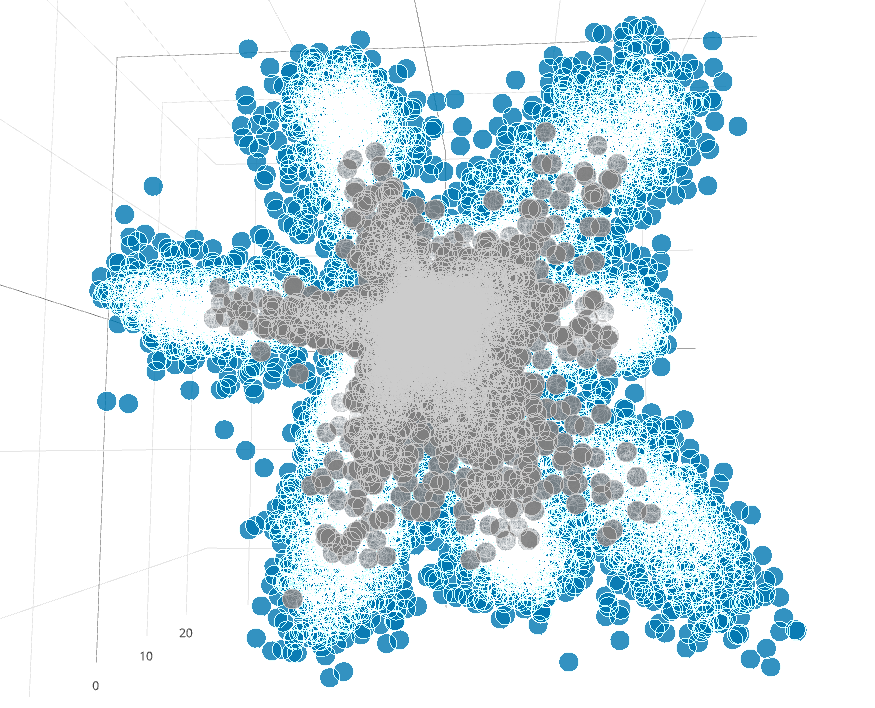
\includegraphics[width=4cm]{MNIST_MNISTM.png} }}%
    \qquad
    \subfloat[Zeros of datasets]{{\includegraphics[width=4cm]{Zeros_MNIST_MNISTM.png} }}%
    \caption{The visualization of samples transformed by feature extractor with output size equals 3. (a) presents two stars formed by samples from source domain (MNIST/blue) and a target domain (MNIST-M/gray) (b) shows how pictures of zeros are mapped - yellow points are zeros from MNIST and green ones from MNIST-M}%
    \label{fig:MNIST_3D}%
\end{figure}

\subsubsection{Conceptors}
\par
Our first approach could be using of conceptor computed with samples from $F_{MNIST}$. As we assume, the conceptor defines an ellipsoid that approximates points cloud from certain distribution. Therefore multiplying some set of points by the concpetor matrix $C_{MNIST}$ would project the set into space of $F_{MNIST}$. Unfortunately in 3-dimensional case, the $C_{MNIST}$ is almost an identity matrix $I_{3}$. We should not be surprised, as our data points cloud is a mulit-armed star and limiting it with an ellipsoid requires it to be a sphere, we cannot approximate those points with any kind of flatten ellipsoid. Moreover, the singular value decomposition (SVD) of conceptor matrix $C$ results in $C = U\Sigma U^{T}$, where $U$ and $U^{T}$ can be interpreted as rotation matrices and $\Sigma$ is a diagonal matrix with singular values of $C$ on diagonal. As all singular values of conceptor matrix are real numbers from $[0,1]$, the conceptor matrix multiplying is in fact rotation, shortening (as non-zero values of $\Sigma$ are $\leq 1$) in certain directions and then re-rotating all the points (see Figure~\ref{fig:ConceptorRotation}). Therefore we cannot transform $F_{MNIST-M}$ to resemble $F_{MNIST}$ with conceptor matrix $C_{MNIST}$, as the multi-amred star formed by points cloud would get even smaller, so it would increase the difference between source and target domains.

\begin{figure}[htb]%
    \centering
    \subfloat[$F_{M}$]{{\includegraphics[width=2.2cm]{C1.png} }}%
    \qquad
    \subfloat[$U^{T} \cdot F_{M}$]{{\includegraphics[width=2.2cm]{C2.png} }}%
    \qquad
    \subfloat[$\Sigma \cdot U^{T} \cdot F_{M}$]{{\includegraphics[width=2.2cm]{C3.png} }}%
    \qquad
    \subfloat[$U \cdot \Sigma \cdot U^{T} \cdot F_{M}$]{{\includegraphics[width=2.2cm]{C4.png} }}%
    \caption{The visualization of transformation points cloud by its conceptor based on SVD of concpetor matrix $C$. The representation $F_{MNIST}$ of MNIST test set (blue points) has firstly been rotated (gray), then scaled (yellow) and finally re-rotated (green)}%
    \label{fig:ConceptorRotation}%
\end{figure}
\par
With this kind of knowledge one thing we can do is transforming points from $F_{MNIST}$ with conceptor matrix $C_{MNIST-M}$ instead of transforming the $F_{MNIST-M}$ with $C_{MNIST}$. As mentioned before, the concpetor matrix is making points cloud tighter, so we could try to take the bigger points cloud (the one corresponding to MNIST) and fit it to the size and shape of the smaller one (see Figure~\ref{fig:ConceptorMnist}). As we already have a well-trained model that performs well in MNIST recognition, we can extend it with a layer with no learnable parameters, that gets the input and multiplies it by conceptor matrix $C_{MNIST-M}$. Formally our model so far is a sequence of a feature extractor $G_{f}$ (with parameters $\Theta_{f}$), 3D mapping and its parameters $\Theta_{3}$ and label classifier $G_{y}$ with parameters $\Theta_{y}$, so the result for input vector $x$ is $G_{y}( G_{3}( G_{f}( x ; \Theta_{f}) ; \Theta_{3} ) ; \Theta_{y} )$. Now we want to freeze the trained feature extractor and 3D mapping (let's call this part of our architecture as $G_{3}$) and multiply its result by $C_{MNIST-M}$, what gives us the new representation ($G_{3} ^ {C} = C_{MNIST-M} \cdot G_{3}$) of the input.
\par
The mapping of points from target domain with $G_{3}^{C}$ compared to transforming source domian with $G_{3}$ is illustrated in the second picture of Figure~\ref{fig:ConceptorMnist}. If the model constructed with non learnable $G_{3}^{C}$ and re-learned $G_{y}$ learns to classify the digits from source domain we would expect the model containing $G_{3}$ and $G_{y}$ perform well on target domain, as the $G_{3}$ transforms MNIST-M to grey points cloud from mentioned picture, so $G_{y}$ should hardly see the difference between domains. After just few epochs the label classifier adjusted to new representation and managed to reach 98\% accuracy on MNIST test set. Now we "unpack" the $G_{3}^{C}$ to $G_{3}$ and check its performance on MNIST-M. The model got 36\% of accuracy, so it improved by 16\% from previous 31\%. We can see the improvement, but we could expect something better, as we forced domains to get really similar.
\par
The last picture of Figure~\ref{fig:ConceptorMnist} presents three points clouds - the blue one is the result of transforming source domain test set with $G_{3}C$. The yellow is target domain test set after transformation by $G_{3}$ (same as grey points from the second picture). The green points cloud is a mapping target domain by $G_{3}^{C}$. As conceptor matrix is making points cloud tighter this distribution was expected. It is worth mentioning that we can easily get a domain predictor $G_{d_{3}}$ that is performing well on both $G_{3}$ and $G_{3}C$ transformation - the accuracy of prediction whether the point belongs to target or source domain (equivalent to determinate if the point with given coordinates is blue or gray if we are considering distribution from first picture of Figure~\ref{fig:ConceptorMnist}) reached 95\%.
\par
If we look closer at the plot of points we could see that many of target domain ones lie closely to the middle of coordinate system, so maybe the mapping works fine for just few examples which forms the multi-armed star, but most of samples are left with poor transformation, which is unclear for label classifier. Therefore after this test we can have few conclusions. Firstly we cannot use our conceptors intuitions from 3-dimensional space in $d$-dimensional one, as in 3D we are not able to approximate the multi-armed star obtained by samples with nothing but sphere. Nevertheless the improvement of predicting labels for target domain after including conceptor layer shows, that we should consider using conceptors during domain adaptation. The density of target domain points near the $(0,0,0)$ shows that those points clouds look similar at the first glance, but we cannot get a good classifier for target domain with this kind of representation. With this knowledge next things we can do to have a better understanding of our problem is trying to get a model with Gradient Reversal Layer in 3-dimensional space, and check the performance of conceptor layer in higher dimensions. Moreover we can check the variant with mapping feature extractor to 2-dimensions to verify all noticed behaviours. 

\begin{figure}[htb]%
\captionsetup[subfigure]{labelformat=empty}
    \centering
    \subfloat[]{{\includegraphics[width=3cm]{Cm(X).png} }}%
    \qquad
    \subfloat[]{{\includegraphics[width=3cm]{Cm(X)_Xm.png} }}%
    \qquad
    \subfloat[]{{\includegraphics[width=3cm]{Conceptor_train.png} }}%
    \caption{Transforming data with conceptor matrix $C_{MNIST-M}$ corresponding to target domain samples. First picture shows the 3D mapping of source domain (blue) and its transformation. The second one presents the transformation $G_{3}C$ of samples form source domain and 3D mapping $G_{3}$ of target domain test set. Last picture shows distributions after training label classifier on $G_{3}C$ mapping - blue points are again transformation of source domain, yellow ones are 3D mapping of target domain (equivalent to grey points from previous picture) and green points cloud is its $G_{3}C$ transformation.}%
    \label{fig:ConceptorMnist}%
\end{figure}

Before changing learning method we can see what happens when we change an activation function. All the plots shows that points cloud for both domains differ in size. One way to limit this magnitude is to use a $tanh$ activation function, which maps the input into $(-1, 1)$. Training model with 3-dimensional layer and $tanh$ activations is even more difficult, I managed to get 78\% accuracy on source domain test set, but it was performing better for target domain than model with $leaky ReLU$ (43\%).  As we can see in Figure~\ref{fig:tanh} the mapped points formed something like a cube. The first plot presents the distribution of samples from source domain. Yellow points are locations of pictures of zero digit. We can see more those clusters on the edges of cube, so they should correspond to different digits. Second plot contains the distribution of target domain (gray). It is hard to find some pattern in them, they seem to be shuffled.

\begin{figure}[htb]%
\captionsetup[subfigure]{labelformat=empty}
    \centering
    \subfloat[]{{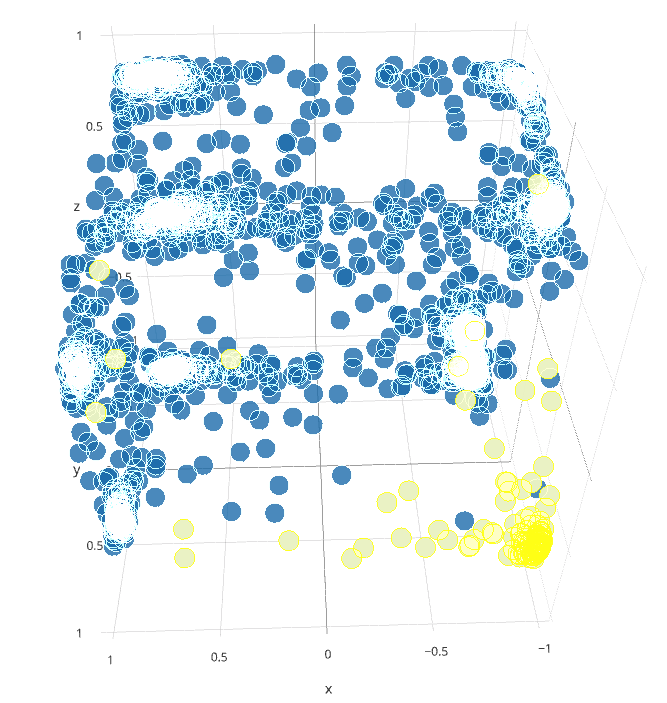
\includegraphics[width=4.5cm]{tanh1.png} }}%
    \qquad
    \subfloat[]{{\includegraphics[width=4.5cm]{tanh2.png} }}%
    \caption{Changing activation function form $leaky ReLU$ to $tanh$}%
    \label{fig:tanh}%
\end{figure}

\subsubsection{Gradient Reversal Layer}
\par
We already know that GRL is a helpful tool in domain adaptation. In higher dimensions models with GRL achieved even 80\% accuracy. There are some approaches using Generative adversarial networks (GAN) that perform even better, so we can still improve our method. Therefore understanding of what really  GRL does is necessary to move on. We can use a model with 3-dimensional feature extractor output then and visualize the results. Now our architecture is not only feature extractor with 3D mapping $G_{3}$ and label predictor $G_{y}$, but also domain classifier $G_{d}$ that is using GRL during training so that representation yielded by $G_{3}$ does not contain information about domain. After a short training I got a model with 96\% accuracy on source domain test set and 40\% accuracy on target domain test set. The improvement is almost 30\% in relation to model without GRL and domain predictor. We can expect now that if we plot the $G_{3}$ mapping of points clouds for source and target domain we should see again two multi-armed stars but more similar than in previous section. 
\par
However the result is really surprising. We can see in Figure~\ref{fig:GRL3D} how samples from source and target domain were transformed. First picture presents the distribution of source domain. It looks similar to the one obtained with model without GRL. The second picture is something we didn't expect - samples from our target domain - MNIST-M formed a blob that is not similar to the source domain distribution at all. When we look at the last picture of the figure we can see the location of samples with label zero. Those from target domain are focused around zeros form source domain, but the matching seems much worse than in model without GRL. Therefore, the reason why GRL is such an improvement becomes even more incomprehensible.

\begin{figure}[htb]%
\captionsetup[subfigure]{labelformat=empty}
    \centering
    \subfloat[]{{\includegraphics[width=3cm]{GRL_3D1.png} }}%
    \qquad
    \subfloat[]{{\includegraphics[width=3cm]{GRL_3D2.png} }}%
    \qquad
    \subfloat[]{{\includegraphics[width=3cm]{GRL_3D3.png} }}%
    \caption{Output of feature extractor mapping when GRL is used during training. First picture presents how source domain samples are transformed. On the second one there are points clouds for both source (blue) and target (gray) domain. Last picture shows how points with 0 label are distributed - yellow come from source domain while green are from MNIST-M}%
    \label{fig:GRL3D}%
\end{figure}
I decided to take a closer look at the training. During the second run model reached even 52\% accuracy on target domain's test set. This result was obtained after second epoch of training, after the last one the model was able to distinguish 47\% of MNIST-M digits. Such a big difference in performance between two runs of the same training for the same architecture shows that with 3-dimensional layer model becomes very unpredictable. I ran the training (for a new instance of architecture) few more times, during third run model reached 47\% accuracy after first epoch but it ends with just 35\%. During next training the loss became NaN so the model crashed. After that I got a model with 55\% accuracy after 5-th epoch out of 10. Next runs also produced very diverse results. Result for source domain kept high during all of them. Figure~\ref{fig:GRL3D_2} presents some results. First two pictures shows the distribution of points for model from second run - the one that reached 52\% accuracy during training and ended with 47\%. We can see that the best model from the training produced the representation closest to the distribution of source domain samples. After whole training the mapping is again very chaotic and noisy. The last picture is a plot from the training with 55\% best and 52\% final accuracy. Although the results are better the points clouds seem to be less suited to the source domain distribution. 

\begin{figure}%
\captionsetup[subfigure]{labelformat=empty}
    \centering
    \subfloat[]{{\includegraphics[width=3cm]{GRL_3D_B1.png} }}%
    \qquad
    \subfloat[]{{\includegraphics[width=3cm]{GRL_3D_B2.png} }}%
    \qquad
    \subfloat[]{{\includegraphics[width=3cm]{GRL_3D_B3.png} }}%
    \caption{Model with GRL during other runs. First two pictures shows plots for model with 52\% accuracy during training and 47\% after last epoch. Yellow points are the final mapping of target domain, grey ones are obtained with feature extractor from model with best accuracy. Blue ones are transformed samples from source domain. Last picture is a corresponding plot for the best obtained model.}%
    \label{fig:GRL3D_2}%
\end{figure}
\par
Every training reached its best accuracy after one of the firsts epochs, that are characterized with lower $\lambda$ coefficient. As $\lambda$ changes nonlinearly from 0 to 1 I decided to use fixed value $\lambda$ during the training. The coefficient was set to 0.3, 0.4 and 0.5. All the models did not managed to get a better performance than already obtained. The accuracy within a single training was also unstable, so fixing $\lambda$ did not make an impact on the research. We are able to make over 50\% improvement with GRL then, but we cannot tell clearly why it works. Figure~\ref{fig:GRL_digits} shows how particular digits were mapped by feature extractor from model with over 50\% accuracy on MNIST-M test set. Each arm of star obtained from source domain samples corresponds to individual digit. In blob formed by target domain test set we can see a cluster for each digit, but it still looks like shuffled. Last picture presents the location of points for both domain in coordinate system. It seems that some of them overlap, what may cause better performance of a classifier.

\begin{figure}%
    \centering
    \subfloat[MNIST mapped]{{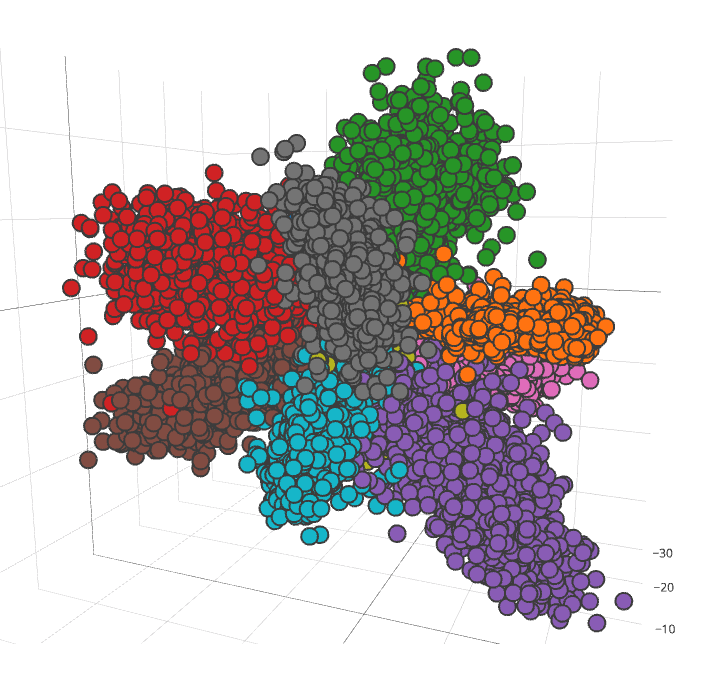
\includegraphics[width=3cm]{GRL_digits1.png} }}%
    \qquad
    \subfloat[MNIST-M mapped]{{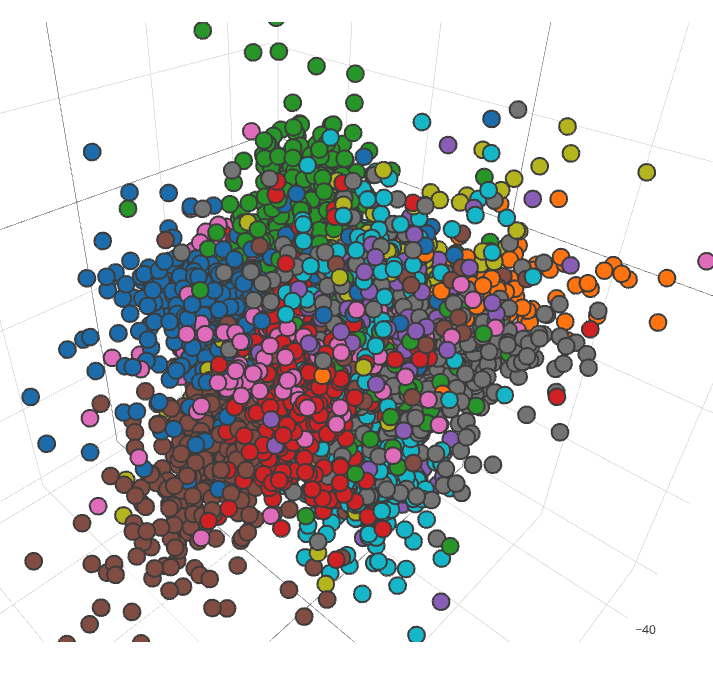
\includegraphics[width=3cm]{GRL_digits2.png} }}%
    \qquad
    \subfloat[Both points clouds]{{\includegraphics[width=3cm]{GRL_digits3.png} }}%
    \caption{Mapping for particular digits. The points clouds are obtained with feature extractor of model that uses GRL during training. Last picture shows how both points cloud are located in 3-dimensional coordinate system.}%
    \label{fig:GRL_digits}%
\end{figure}
\subsubsection{2-dimensional case}
\par
Visualization with digit division is a good way to understand what really happens during training. To make plots even more understandable we can change our feature extractor to map output into 2-dimensional space. Although finding right parameters gets more difficult, after few epochs of training we can get a model with 95\% accuracy for source domain (MNIST) and 31\% for samples from MNIST-M. These results are satisfying as we are asking our model to pack all the crucial information about 28x28 pixel photo into 2 real numbers. First two pictures of figure~\ref{fig:2D} presents the transformation of MNIST and MNIST-M test sets. Each point is a mapping of input image with digit corresponding to point's color. MNIST samples are formed into 7-armed star, each for different digit. Input images for 3 digits (3,5,8 in this case) are stacked in the middle, which does not interfere with good classifier performance. Samples from target distribution also formed similar 7-armed star but, like mentioned before, a large number of them was mapped near the middle of coordinates system. This characteristic is more clearly visible in 2-dimensional case. As input images for different digits are represented by similar numbers the classifier cannot be sure while predicting the label.
\par
We can also apply a training with Gradient Reversal Layer for this architecture. Just like before the source domain samples are mapped into multi-armed star and visualization of points cloud obtained by mapping the target domain resluts with a plot of huge blob (last picture of figure~\ref{fig:2D}). The performance of this model is better thanks to the use of a GRL, but I could not get any new useful knowledge from this research. Also trying to improve the model's performance with conceptor did not succeed. As in the 3-dimensional case the conceptor of our mapped set of points is an ellipse that is limiting the points cloud. Here we can see that it would be difficult to approximate our samples by something but a circle, hence the conceptor matrix is almost an identity matrix. Therefore filtering the point by the matrix hardly changes its coordinates. Once again I must point out that we cannot be sure taht this behaviour of conceptor would happen in higher dimension.

\begin{figure}[htb]%
\captionsetup[subfigure]{labelformat=empty}
    \centering
    \subfloat[]{{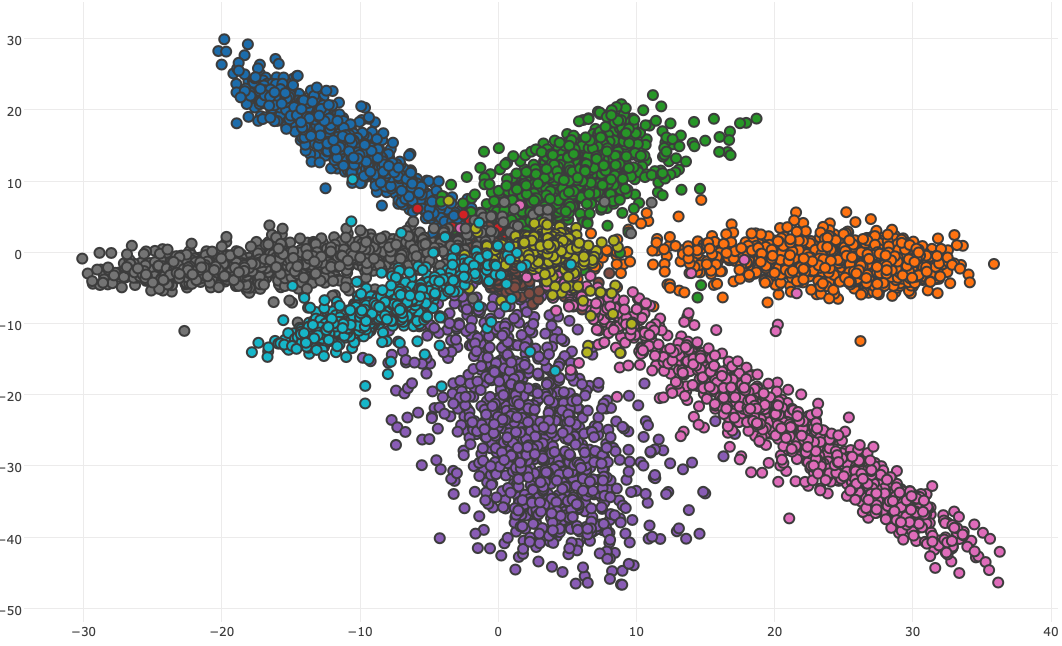
\includegraphics[width=3cm]{MNIST_2D.png} }}%
    \qquad
    \subfloat[]{{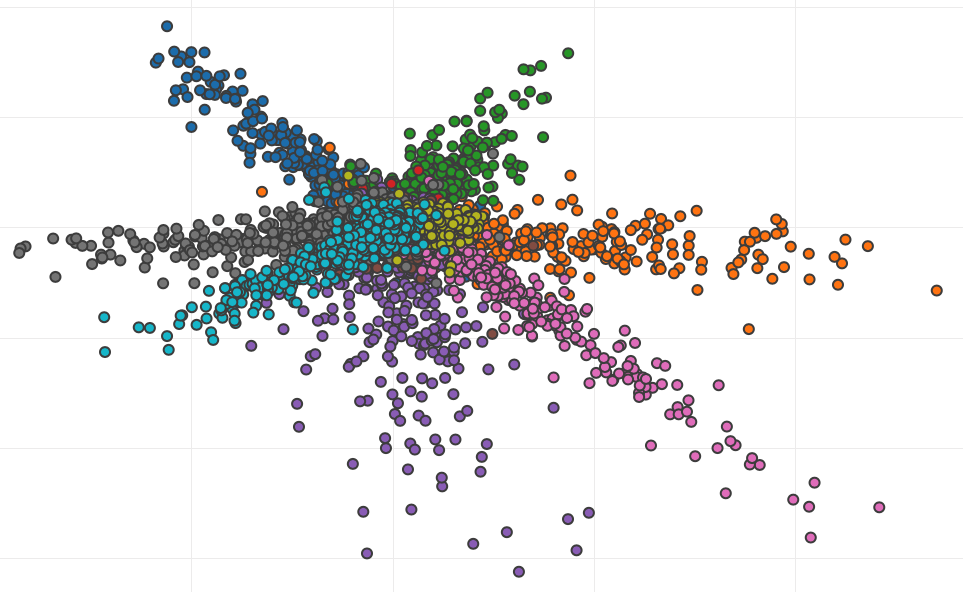
\includegraphics[width=3cm]{MNIST_M_2D.png} }}%
    \qquad
    \subfloat[]{{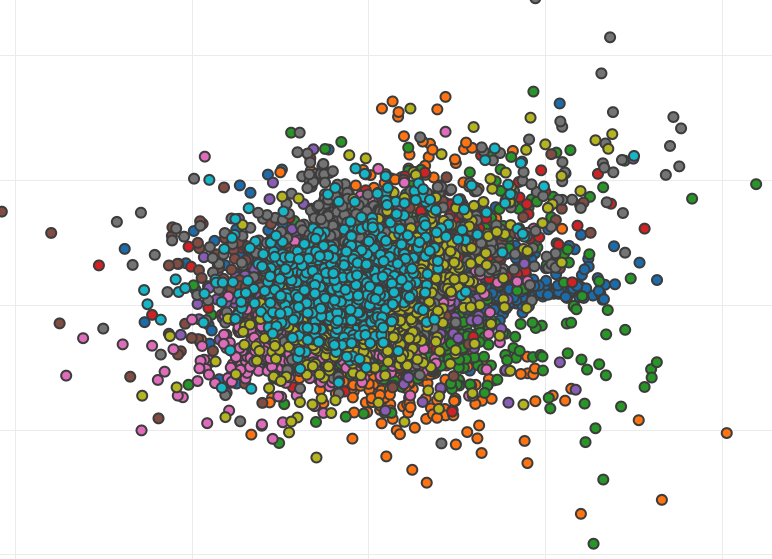
\includegraphics[width=3cm]{MNIST_M_2D_GRL.png} }}%
    \caption{Mapping for particular digits with feature extractor yielding 2-dimensional vector. First picture shows the distribution for samples from source domain, second one for input from target domain and the last one is a mapping of target domain samples after training with GRL applied.}%
    \label{fig:2D}%
\end{figure}

\subsection{SVHN and MNIST}
\par
All previous observations were made for highly correlated source and target domain, as MNIST-M is obtained with MNIST dataset. To be sure that results of the research is not caused by the connection between MNIST and MNIST-M we should try to run the experiments for some other domain. Once again I used SVHN dataset as a source domain and tried to improve its performance in MNIST digit recognition. 
\subsubsection{Model without Gradient Reversal Layer}
\par
Firstly let's try to get a model with 3-dimensional layer, that is performing well on SVHN classification. As predicting the label for samples from SVHN dataset is a way harder task than MNIST recognition the model must be more complicated and the task of learning architecture witch such a small layer inside may failed. Fortunately model with a complex feature extractor that was used previously to tune parameters for SVHN classifier succeed in learning task. After few epochs it reached 92\% accuracy on source domain (SVHN) test set and 65\% on target domain (MNIST) samples. The performance on MNIST test set is satisfying, it seems that we did not lose many information during mapping a vector transformed by feature extractor to 3-dimensional space, as without this layer we can get a model with just slightly better results (94\% accuracy for source domain, 70\% for the target one). Now let's look at the visualization of mapping a set of samples from both domains. As in previous section I used MNIST test set $MNIST_{T}$ (never seen by any architecture neither with GRL nor without) and $SVHN_{T}$ - 10000 randomly sampled images from SVHN test set. The feature extractor with 3D mapping is denoted again as $G_{3}$ - note that it is much more complex than $G_{3}$ from previous section. The points clouds obtained by mapping those input vectors sets are $F_{SVHN} = \{ G_{3}(x) | x \in SVHN_{T} \}$  and $F_{MNIST} = \{ G_{3}(x) | x \in MNIST_{T} \}$.   

\begin{figure}%
    \centering
    \subfloat[SVHN]{{\includegraphics[width=3cm]{SVHN.png} }}%
    \qquad
    \subfloat[SVHN and MNIST]{{\includegraphics[width=3cm]{SVHN_and_MNIST.png} }}%
    \qquad
    \subfloat[Zeros of datasets]{{\includegraphics[width=3cm]{Zeros_SVHN_MNIST.png} }}%
    \caption{The visualization of samples transformed by feature extractor with output size equals 3. (a) presents the star formed with samples from source domain (SVHN), (b) shows how data from target domain is mapped and (c) where zeros for both domains lie in the space}%
    \label{fig:SVHN_3D}%
\end{figure}
\par
First picture of figure~\ref{fig:SVHN_3D} presents the distribution of $F_{SVHN}$. The samples from SVHN domain formed a solid resembling a multi-armed star, that looks much more sharper than the one obtained in previous section, when model was trained on MNIST dataset. Second image shows the relation between $F_{SVHN}$ (blue) and $F_{MNIST}$ (gray). Samples from target domain are formed in a very similar multi-armed star, even the magnitude of the solid is close to the one composed of SVHN input images. In the previous MNIST/MNIST-M section, the improvement of the model was correlated with reducing the difference in size of obtained points clouds, therefore the good performance of classifier on target domain is understandable. Last picture of the figure shows the positions of images of zero digit from both domains. For source domain our $G_{3}$ mapping found a way to form every digit into individual arm of the star. When we transform zeros from $MNIST_{T}$ with this mapping we can see that they are scattered over two arms of obtained star, also many of them lie in the middle of the solid. It causes the label prediction imprecission, as samples with different labels are mixed. Figure~\ref{fig:SVHN_Digits} shows how every of 10 digits was distributed by $G_{3}$. Samples from source domain are well-formed in distinguishable arms of our star. In the target domain case we can also assign every arm of obtained solid to different label, but we can see that some of samples lie far from cluster formed by images with the same digit.

\begin{figure}[htb]%
    \centering
    \subfloat[$F_{SVHN}$]{{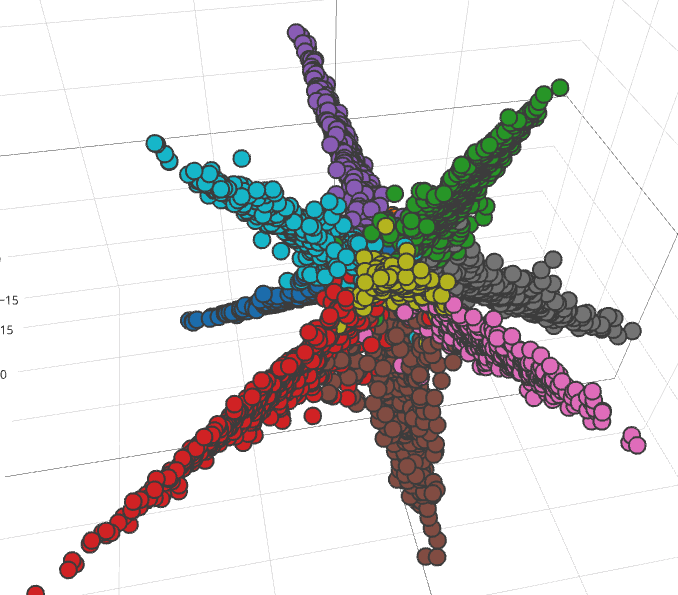
\includegraphics[width=4.5cm]{SVHN_digits1.png} }}%
    \qquad
    \subfloat[$F_{MNIST}$]{{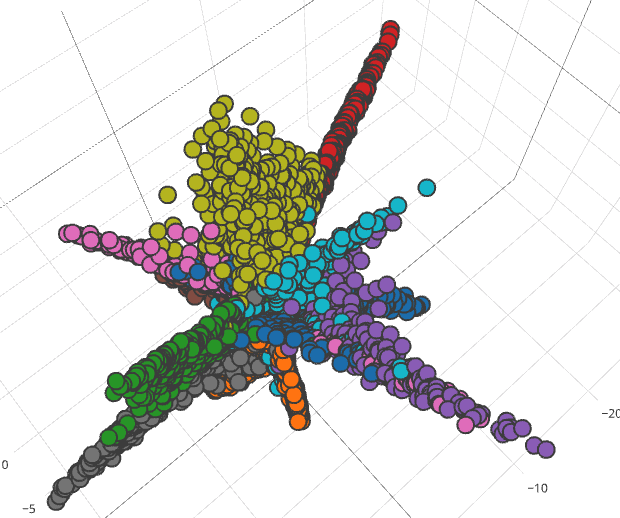
\includegraphics[width=4.5cm]{SVHN_digits2.png} }}%
    \caption{Distribution of particular digit images after $G_{3}$ mapping.}%
    \label{fig:SVHN_Digits}%
\end{figure}

\subsubsection{Model with Gradient Reversal Layer}
\par
We already know that training a model with a Gradient Reversal Layer and 3-dimensional layer is much more complicated. Although I managed to get a well-tuned network in previous section, when I added a domain predictor $G_{d}$ with GRL inside I was unable to train a newly initialized model, during whole training the loss did not reduce so accuracy on test sets of both source and target domain was the same as for random model. This shows that the task became too complex, no model was able to pack all the crucial information in just three numbers while GRL was used. 
\par
One thing that came to my mind was to get the pre-trained model that did not use GRL, like the one from previous subsection, and add the domain predictor with GRL to it. This approach was partly successful, as after third epoch of new training (with GRL) the model reached 72\% accuracy on $MNIST_{T}$. Unfortunately at the begining of next epoch the loss value became NaN, so the model got useless. As the $\lambda$ coefficient is getting larger over the epochs I decided to fix it to a certain, lower value during whole training. With $\lambda$ set to 0.4 and 0.2 the pre-trained model improved in MNIST recognition to 73\%, so the GRL improved the performance by 12\%. The result is quite good, as without limiting the size of any layer I did not get much better. Figure~\ref{fig:SVHN_GRL} presents the distribution of $F_{MNIST}$ after training the model with Gradient Reversal Layer. Distribution from first picture was obtained with model that tuned $\lambda$ during training, the parameters of used $G_{3}$ were serialized before the loss got NaN. Second picture is plot of transformation $MNIST_{T}$ with model that used $\lambda = 0.2$ during whole training. The result for $\lambda = 0.4$ is very similar, so there is no point in including the plot. In both pictures we can see that there are less points located in wrong arm of the star. This obviously leads to the better performance of the classifier. Unlike a MNIST/MNIST-M training case the obtained points cloud is recognizing the shape from no-GRL training. However in previos section we trained the model from the begining, here we use a pre-trained one and the $\lambda$ is set to a low value, so the mechanism of Gradient Reversal Layer has less impact on transformation of input vector.
\par
You can wonder if the multi-armed star look of samples from target domain is really caused by the relation between domains - both are images of digits, or if the shape has nothing to do with the domain shift and all those observations are pointless. To verify it I created a random dataset with samples of size equal to the size on SVHN image and values distributed form $\mathcal{N}(\mu_{SVHN},\,\sigma_{SVHN}^{2})$, where $\mu_{SVHN}$ is just the values' of pixels mean SVHN images and $sigma_{SVHN}^{2}$ their variance. The visualization of mapping this dataset with $G_{3}$ was just a blob of points, so we cannot suppose that the multi-armed star is not related with images of digits.

\begin{figure}[htb]%
\captionsetup[subfigure]{labelformat=empty}
    \centering
    \subfloat[]{{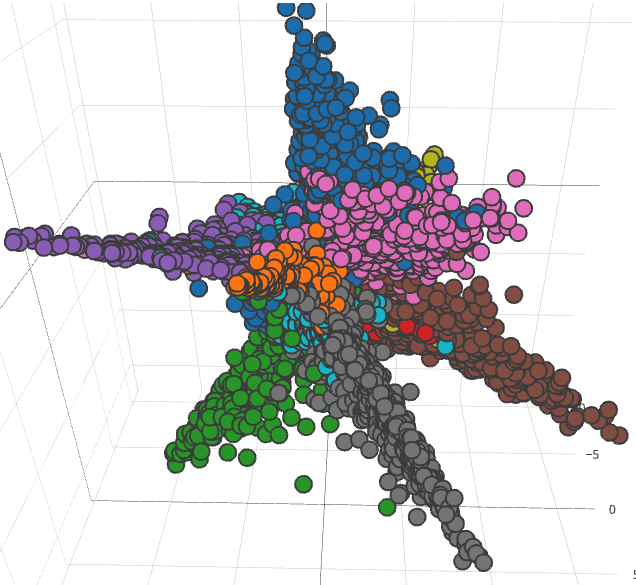
\includegraphics[width=4.5cm]{SVHN_GRL.png} }}%
    \qquad
    \subfloat[]{{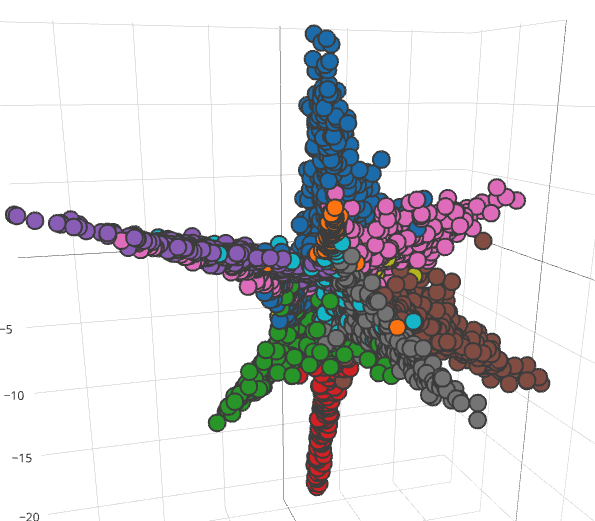
\includegraphics[width=4.5cm]{SVHN_GRL2.png} }}%
    \caption{Distribution of particular digit images after $G_{3}$ mapping with GRL used during training.}%
    \label{fig:SVHN_GRL}%
\end{figure}

\subsection{Higher dimension performance}
\par
During studying the dependence between MNIST and MNIST-M we could see that adding the conceptor computed for target domain to our feature extractor and then re-tuning the label predictor can improve the result of classifier for target samples, as the new classifier has its input more related with target domain distribution. To check if this behavior occurs in higher dimension I trained the model without 3-dimensional layer and ten add the conceptor matrix $C$ multiplication to the feature extractor $G_{f}$ output. Then the label predictor $G_{y}$ was trying to predict the digit for representation $G_{f}^{C}(x)$ of input vector $x$. Just like in 3-dimensional case there was no problem for $G_{y}$ to adjust to the new input distribution. After the training I unpacked $G_{f}^{C}$ to $G_{f}$ and checked the performance of the model. In contrast to the model with 3-dimensional layer inside, this time there was no improvement on target domain test set. This results show that it is hard to get the intuition about how conceptors really word with 3-dimensional mapping of such complex data.

\end{document}
